\chapter{\label{intro}Introduction}
%%%%%


\Glspl{GW} were first predicted in 1915 as a consequence of Einstein's general
theory of relativity \citep{einstein2005GrundlageAllgemeinen}, where they were
theorised as ripples in the fabric of space-time.  this would open up a new window into the universe which is not accessible via electromagnetic observations. 
The first observational evidence that \glspl{GW} exist came from observations of the Hulse-Taylor
binary \citep{weisberg1981GravitationalWaves,weisberg2004RelativisticBinary}, which subsequently won the Nobel prize in 1993.
This observation, which was of a pulsar in a binary system showed that the periastron was
reached slightly early after each orbit, implying that the pulsars orbital radius was
decreasing with time.  If the separation of two orbiting objects is decreasing
then the system must be losing energy.  The loss in energy matched the \gls{GR}
prediction which assumed the energy was lost to \glspl{GW}, giving hope of
the existence of \glspl{GW} and motivating the design of instruments
which could directly detect them.

The first direct detection of gravitational
waves was made in 2015 when the two \gls{LIGO} detectors in the US
\citep{abbott2016ObservationGravitational} identified a signal from a \gls{BBH}
system.  This was not only the first observation of a \gls{GW} but gave
information on an as yet unobserved type of astrophysical
system.  This has since been followed by many more detections of \gls{BBH}
signals, including those from a three detector network (the two \gls{LIGO} detectors and Virgo)
\citep{abbott2017GW170814ThreeDetector,theligoscientificcollaboration2020GW190425Observation}, which allowed better localisation of the source on the sky.  
In 2017 the \gls{LIGO} detectors observed the
first \gls{BNS} system \citep{abbott2017GW170817Observation} where a
corresponding electromagnetic counterpart was also observed.
This allowed verification~\chris{what does verification eman in
this sense?} of the source from optical counterparts and started the era of
multi-messenger astronomy.  These detections opened up the field of
\gls{GW} astronomy, where many more detections are expected to give more
information on the universe and objects within it.

As well as searching for \gls{BBH} and \gls{BNS} signals, there are many
efforts to detect other types of \gls{GW} signals.  This thesis focuses on
efforts to search for a particular type of \gls{GW} which are thought to
originate from rapidly rotating neutron stars.  In chapters \ref{intro} and
\ref{searchcw} I will review introductory material.  This includes a general
introduction to the generation of \glspl{GW} in Sec.~\ref{intro:gravwaves} and
their sources in Sec.~\ref{intro:sources}.  I will then introduce instruments
used to detect \gls{GW} in Sec.~\ref{intro:detector}.  In Chapter
\ref{searchcw} I will introduce the general model for \glspl{CW} and current
methods used to detect them.  Chapters \ref{soap}, \ref{machine} and
\ref{detchar} will go into detail about techniques developed by the author to
search for \gls{CW} signals.  Finally I will summarise this work and discuss
future developments in chapter \ref{summary}
~\chris{This is a very short introduction to the thesis. This is your
opportunity to lay the ground work (in a non-technical way) before you get into
the details. You could really expand upon the ideas mentioned here. What else
can you say about GWs? What else can you say about the Hulse-Taylor Pulsar
(they won a Nobel Prize), what else can you say about 150914 and 170817? Prove
to the examiner that you are an expert in the general field of GW astrophysics.}

%%%%%%%%%%%
%%%%%%%%%
\section{\label{intro:gravwaves}Gravitational waves}
%%%%%%%%%%%
%%%%%%%%%

In general relativity, gravity is thought of as the curvature of space-time, where
matter moves according to this curvature. Matter also has
an effect on the curvature itself, where larger masses will distort space-time more than smaller masses. 
To describe space-time, one would want to link the curvature to the matter mathematically, this was done in 1915 \citep{einstein2005GrundlageAllgemeinen} where Einstein developed his field equations
\begin{equation}
\label{intro:gravwaves:efe}
    G_{\mu \nu} = \frac{8 \pi G}{c^4}T_{\mu \nu}.
\end{equation}
where $G_{\mu \nu}$ is the Einstein tensor, $G$ is the gravitational constant, $c$ is the speed of light and $T_{\mu \nu}$ is the
stress-energy tensor.  The stress energy tensor contains information on the density and flux of energy and momentum at a given point in space-time.  
The Einstein tensor contains information on the curvature of the
universe, which can be derived directly from the metric tensor $g_{\mu \nu}$
which describes the space-time geometry.
Einstein's equations then explain how the curvature of space-time changes with
the mass-energy within it.  

In empty space, i.e $T_{\mu \nu} = 0$, one can assume that the geometry of space-time is flat, i.e. there is no curvature to space-time. The metric tensor for flat space is defined as
\begin{equation}
    \label{intro:gw:minkowski}
g_{\mu \nu} = \eta_{\mu \nu} = \left(
\begin{matrix}
-1 & 0 & 0 & 0 \\
0 & 1 & 0 & 0 \\
0 & 0 & 1 & 0 \\
0 & 0 & 0 & 1 
\end{matrix}
\right).
\end{equation}
Each index of this matrix refers to a space-time dimension, i.e. $x^0 = t$,
$x^1=x$, $x^2=y$ and $x^3=z$.  Measuring a distance $dx$ in space-time can be
different for different observers, therefore, one needs a measure which is
invariant for every observer.  This is the space-time interval $ds$, also known
as the line element, between two `events' in space-time, which is defined as
\begin{equation}
\label{intro:lineelement}
    ds^2 = g_{\mu \nu} dx^{\mu}dx^{\nu}.
\end{equation}
This equation is a sum over the indices $\mu$ and
$\nu$.  
Equation \ref{intro:lineelement} can be
thought to describe the space-time `distance' between the two events.  For flat
space-time, $\eta_{\mu\nu}$, Eq.~\ref{intro:gw:minkowski} and \ref{intro:lineelement} can be combined to find the space-time interval
%
\begin{equation}
    ds^2 = -c^2 dt^2 + dx^2 + dy^2 + dz^2.
\end{equation}
%
The Einstein equations defined in Eq.~\ref{intro:gravwaves:efe}
then demonstrate how the curvature of space-time $G_{\mu\nu}$ depends on the
matter and energy distribution $T_{\mu \nu}$ within it.~\chris{I think that
there are enough steps missing between defining G from g that this last
statement doesn't really explain how the interval gets us from Minkowski to
space-time curvature.}

A \gls{GW} is then a wave which propagates through space-time, where the simplest way to
visualise this is just a small time dependent change to the flat space-time
metric $\eta_{\mu\nu}$.  In the linearised theory of gravity, the
space-time metric $g_{\mu \nu}$ can be defined as
\begin{equation}
\label{intro:gravwave:metric}
    g_{\mu \nu} = \eta_{\mu \nu} + h_{\mu \nu},
\end{equation}
where $ \eta_{\mu \nu}$ is the metric for flat space-time and $h_{\mu \nu}$ is
some perturbation, where $|h_{\mu \nu}| \ll 1$
\citep{flanagan2005BasicsGravitational}. In the regime of small perturbations, it can be shown that the solutions are plane waves,
more information on this derivation can be found in
\citep{flanagan2005BasicsGravitational,letiec2016TheoryGravitational}.  

By using $g_{\mu \nu}$ from Eq.~\ref{intro:gravwave:metric}, we can write the
linearised Einstein equations as
\begin{equation}
\label{intro:lineinstein}
    \Box h_{\mu \nu} = -16 \pi T_{\mu\nu},
\end{equation}
where $\Box$ is the d'Alembert operator defined by
\begin{equation}
		\Box = -\frac{1}{c^2} \frac{\partial^2}{\partial t^2} + \frac{\partial^2}{\partial x^2} + \frac{\partial^2}{\partial y^2} + \frac{\partial^2}{\partial z^2}
\end{equation}
In empty space there is no matter, therefore, all the components of the stress
energy tensor are zero, i.e. $T_{\mu \nu} = 0$.  This allows
Eq.~\ref{intro:lineinstein} to be reduced to
\begin{equation}
    \Box h_{\mu \nu} = 0,
\end{equation}
which is of course the wave equation.  This follows the same form as in
electrodynamics and the general plane-wave solutions have the form
\begin{equation}
    h_{\mu\nu} = A_{\mu\nu}e^{ik_{\alpha} x^{\alpha}},
\end{equation}
where each component of $h_{\mu \nu}$ is a sinusoid traveling along vector
$\mathbf{k}$ with amplitude $A_{\mu\nu}$
\citep{capano2011SearchingGravitational}. 

At this point the set of equations are not simple; the symmetric tensor $A_{\mu \nu}$ has 10 independent
components~\chris{why is it symmetric? It is, but why?}. This can be greatly
simplified by choosing a different gauge where the metric perturbation is both
transverse and traceless (TT) \citep{flanagan2005BasicsGravitational}.  This is
just a choice of coordinate system which does not change any current
assumptions. This gauge imposes two conditions: one
is that $h_{\mu \nu}$ is traceless, i.e. that the sum of the diagonal elements
are 0 and the other is that $h_{\mu \nu}$ is transverse.  The transverse
element means that the oscillations of the wave happen perpendicular to the
direction of travel.  At this point we can choose that the wave is travelling in
the $z$ direction which means that $k = (\omega,0,0,k)$.  By then adopting the
TT gauge there are only two unique components to the metric such that the
perturbation is
\begin{equation}
\label{intro:gw:gravwave}
h_{\mu \nu} = \left( 
\begin{matrix}
0 & 0 & 0 & 0 \\
0 & h_{+} & h_{\times} & 0 \\
0 & h_{\times} & -h_{+} & 0 \\
0 & 0 & 0 & 0 \\
\end{matrix}
\right) 
e^{i(kt - wt)}.
\end{equation}
The two unique components are then the two polarisations of gravitational
waves, $h_{+}$ and $h_{\times}$. The effect of each of the polarisations can be seen when acting on a ring of independent test masses shown in Fig.~\ref{gw:polarisations}, where in this example the \gls{GW} is travelling out of the page along the $z$ axis.
From Eq.~\ref{intro:gw:gravwave} one can see that the $h_{+}$ component causes space-time to be stretched in the $x$ axis and compressed in the $y$ axis before returning to normal then stretching in the $y$ axis and compressing in the $x$ axis. This can be seen as the test masses being distorted into an ellipse with the semi-major axis along the $x$ or $y$ axis.
The cross polarisation has a similar affect to the plus polarisation but is rotated 45 degrees.
%
\begin{figure}[h]
    \centering
    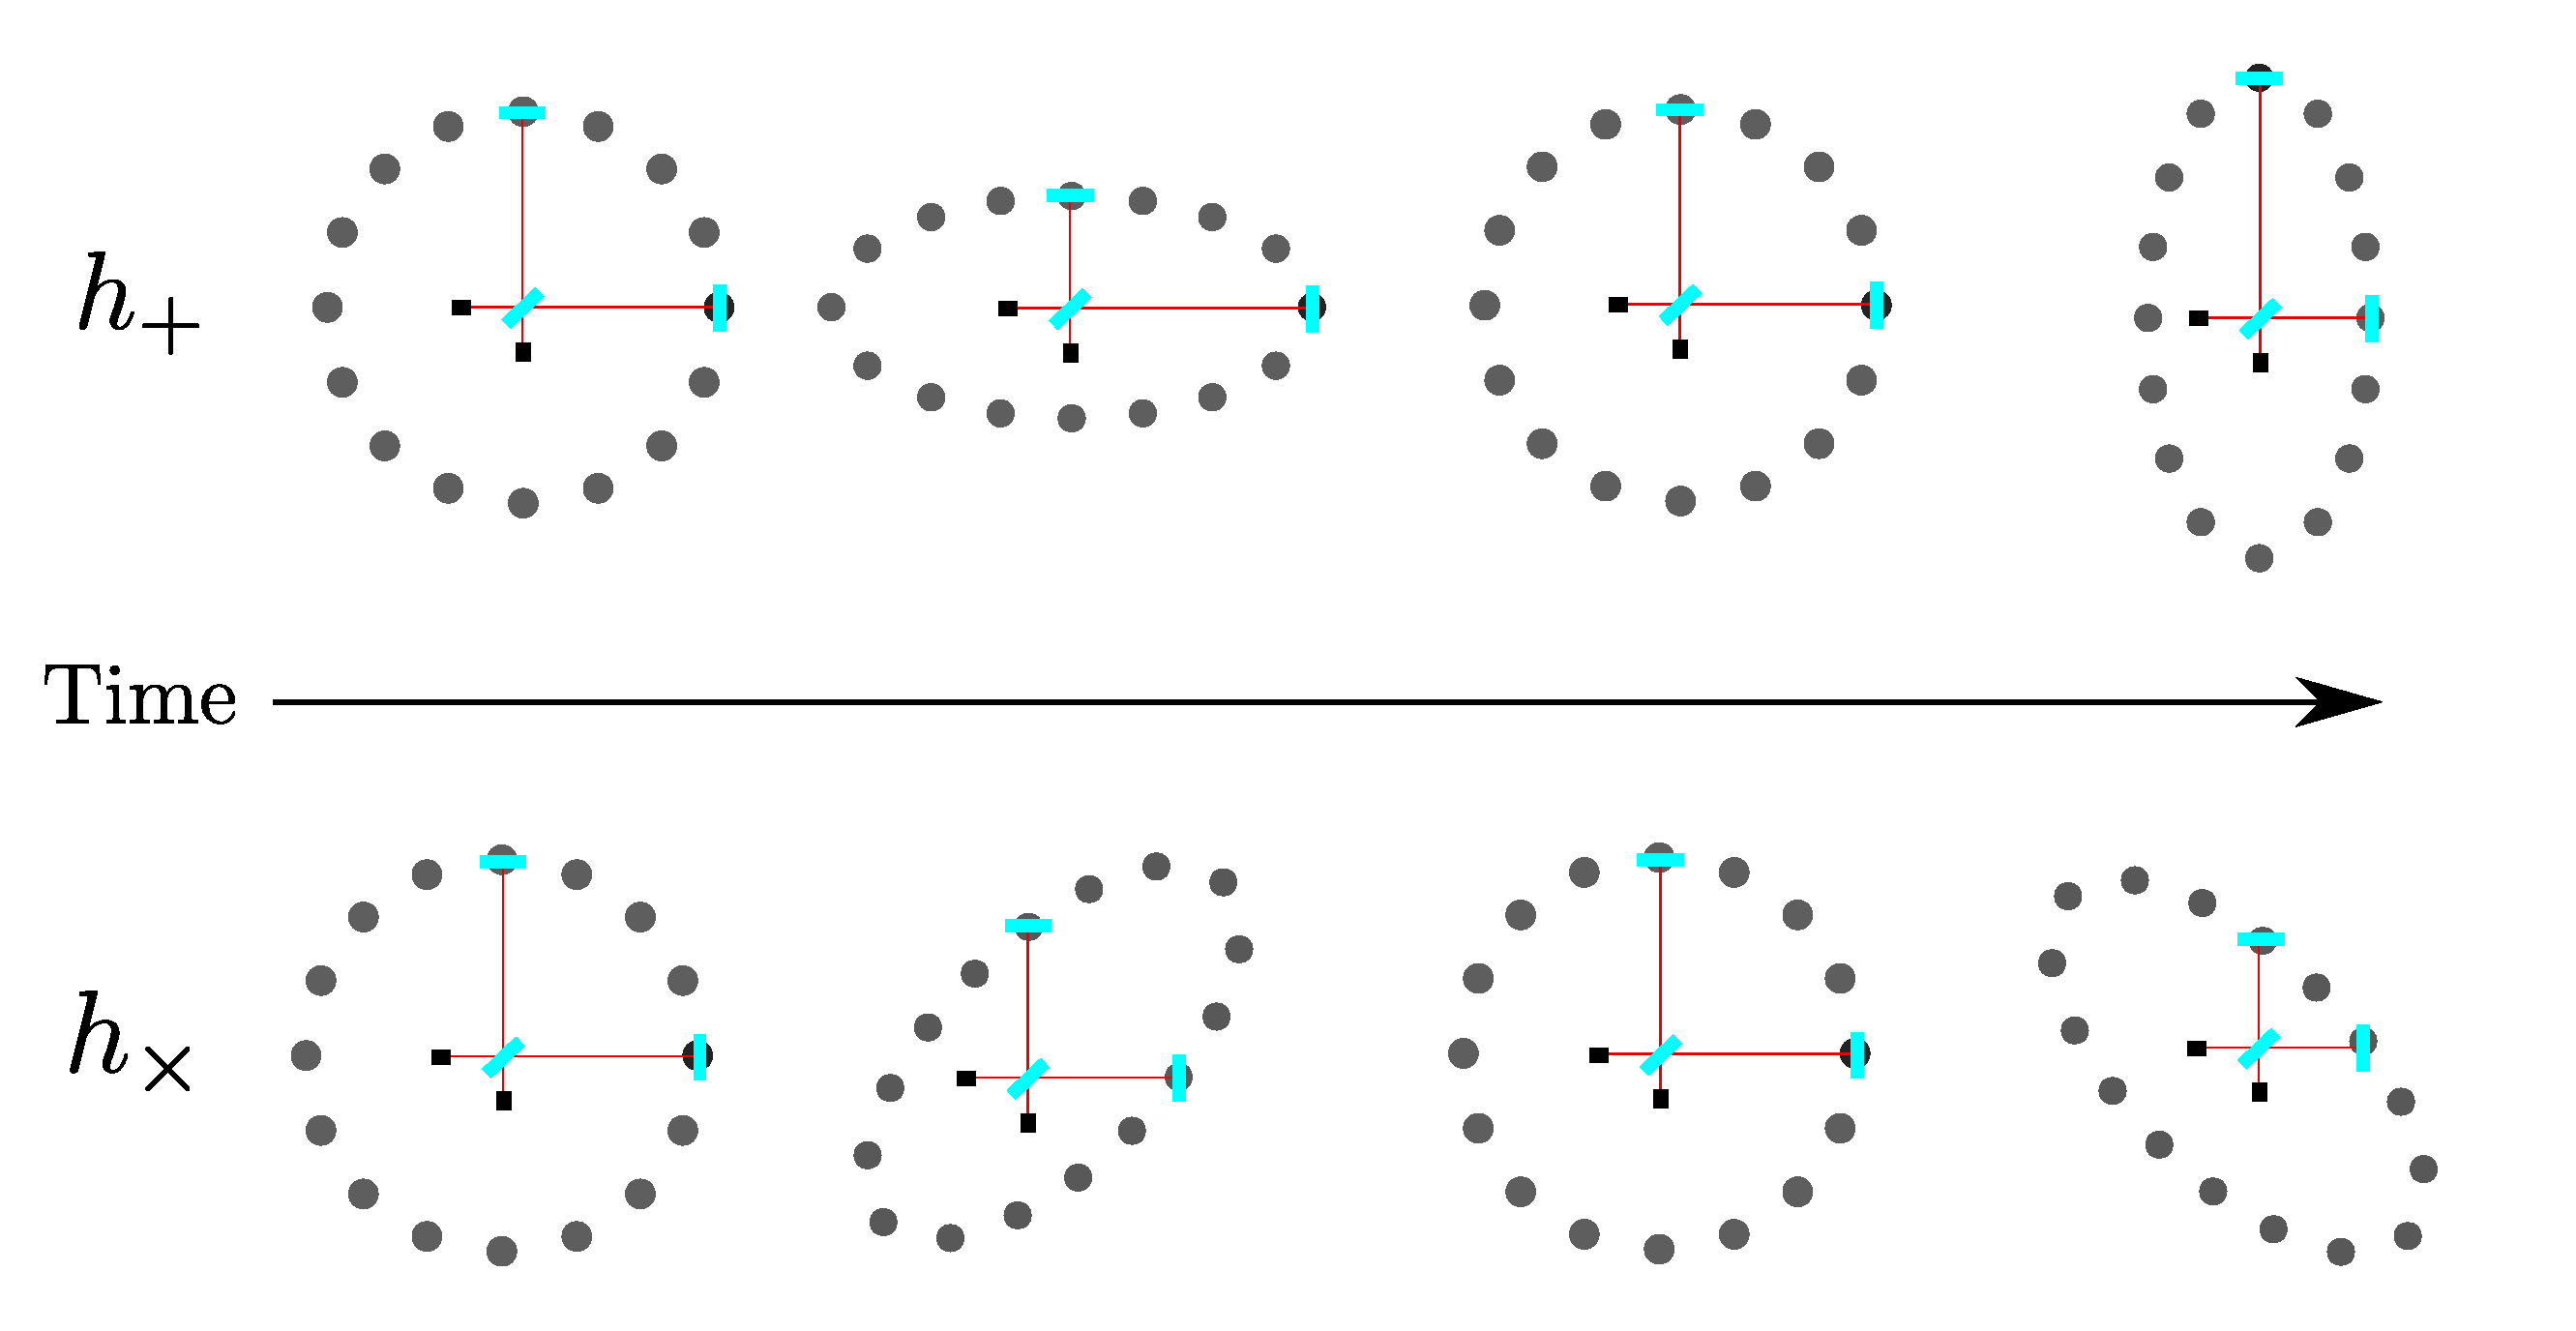
\includegraphics[width=\textwidth]{C1_intro/polarisation_ring.pdf}
 \caption[Plus and Cross polarisations]{These diagrams show how the plus and cross
polarisations affect a ring of test particles. This assumes
the \gls{GW} is travelling out of the page, where the effects
have been greatly exaggerated. This also shows an example of how this
affects the test masses of an interferometer. This will be
described in more detail in Sec.~\ref{intro:detector}.}
\label{gw:polarisations}
\end{figure}



\subsubsection{Generating gravitational waves}

To generate \gls{GW} we can follow the derivation in \citep{flanagan2005BasicsGravitational}, where one can solve Eq.~\ref{intro:lineinstein} to find the \gls{GW} perturbation $h_{\mu \nu}$.
The result of this is that $h_{\mu \nu}$ is related to the second moment of the mass distribution by
\begin{equation}
    \label{intro:gravwave:amp}
        h_{\mu \nu} = \frac{2}{r}  \frac{d^2}{dt^2} Q_{\mu \nu}(t-r),
\end{equation}
where $r$ is the distance from the source \citep{letiec2016TheoryGravitational} and $Q_{\mu \nu}$ is the second moment of the mass distribution defined by 
\begin{equation}
    Q_{\mu \nu}(t) = \int \rho(t,{\bf x}) x^\mu x^\nu d^3x,
\end{equation}
where $\rho$ is the mass density ~\citep{flanagan2005BasicsGravitational} \joe{double check here/reread}.  
This has a slight modification in the TT gauge, see
\citep{flanagan2005BasicsGravitational}, however, has the same relationship
between the mass quadrupole and the \gls{GW} amplitude.  This shows that for
\gls{GW} to be generated, the second derivative of the mass quadrupole moment
is needed. 
Gravitational monopole and dipole radiation is not possible due to the conservation of energy and momentum respectively \citep{misner1973Gravitation} and radiation can be emitted from higher orders but is generally weaker than quadrupolar radiation. \joe{want to say a little more here}

There are many types of system which could emit quadrupole \glspl{GW}, including supernovae, colliding objects and orbiting black holes. 
Typically these are from high mass systems as large amount of energy are needed to overcome the stiffness of space-time which is defined by the $8 \pi G/c^4$ in Eq.~\ref{intro:gravwaves:efe}.
Some of the primary sources of \gls{GW} that are currently searched for will be described in the following section.




%%%%%%%%%%%%%%
%%%%%%%%%%%%%
\section{\label{intro:sources}Sources and signals}
%%%%%%%%%%%%%%%
%%%%%%%%%%%%%%%

There are many potential sources for \gls{GW}, which can be split into 3
general categories based on their signal type: \gls{CBC}, Burst, Stochastic and
\glspl{CW}.  These categories are chosen based on the length of the signal and
how well modelled the signal is.  Figure \ref{intro:sources:signaltypes} shows
an example of each of the signals and their category.
%
\begin{figure}[h]
    \centering
    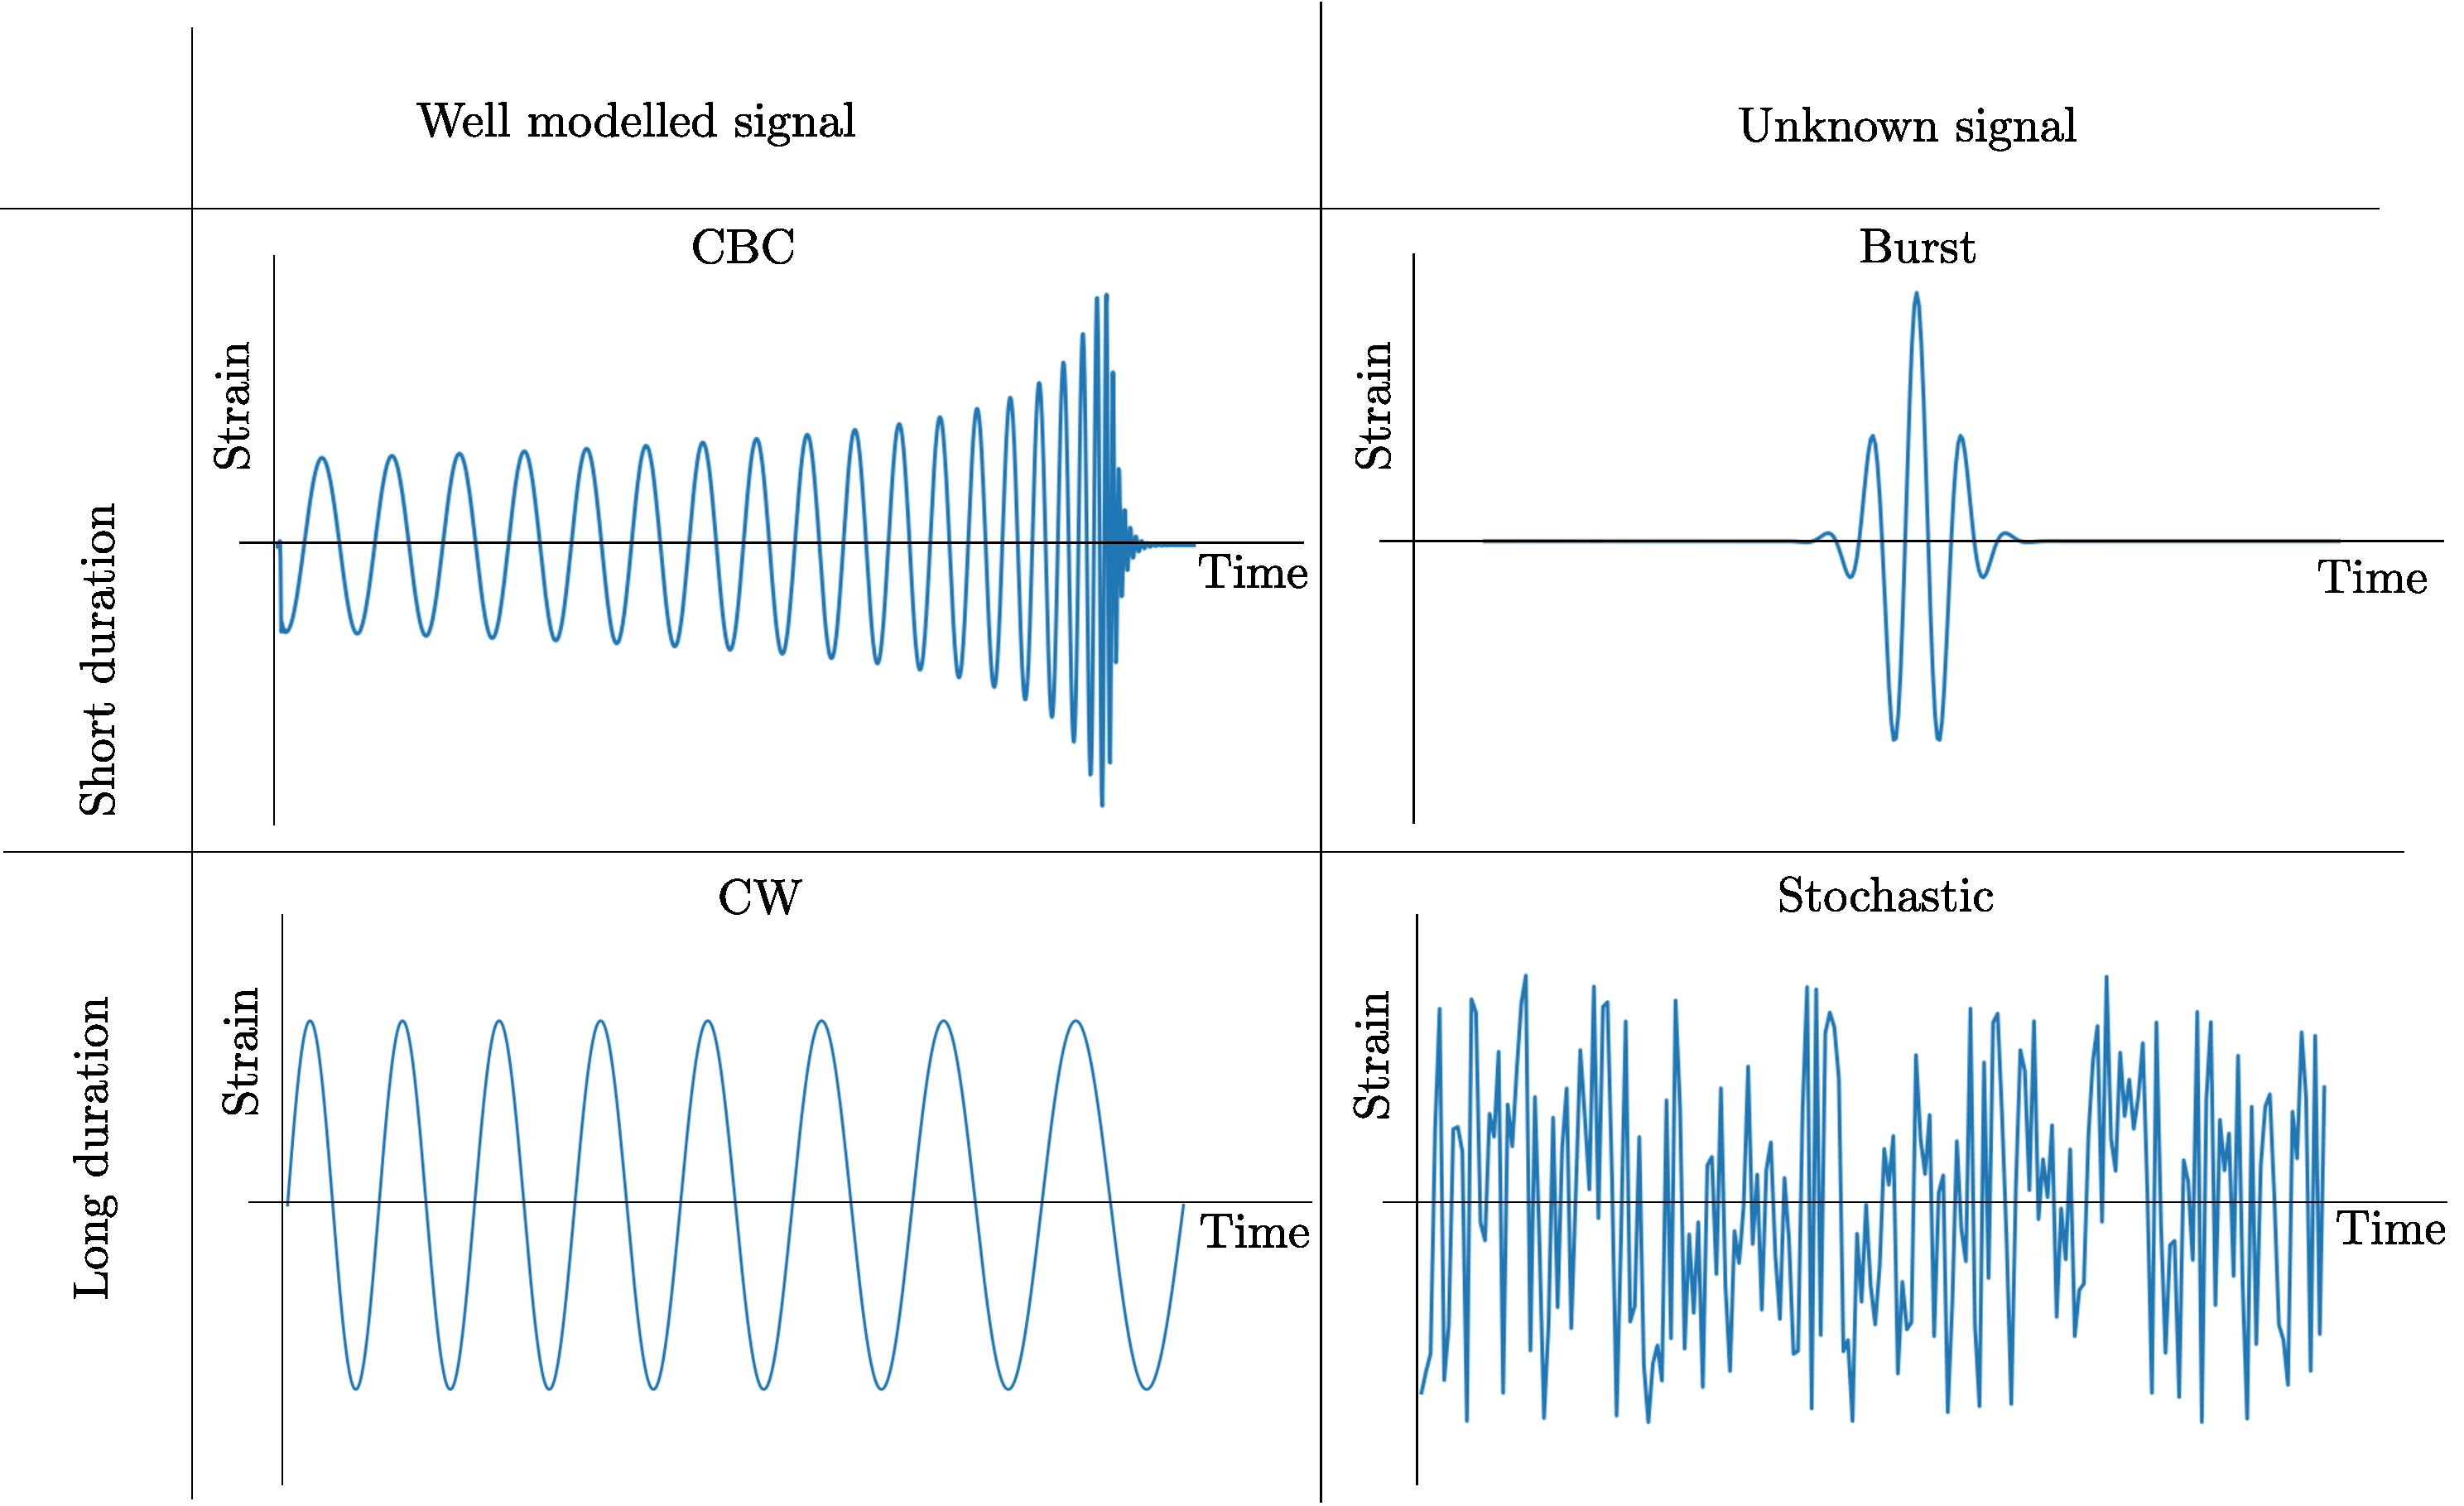
\includegraphics[width=\textwidth]{C1_intro/sources_types.pdf}
    \caption[GW signal types]{Each \gls{GW} signal type can be categorised
based on its signal length and how well the signal is modelled. Transient
signals which are short duration in the ground based detector band, include
both well modelled \gls{CBC} signals and unknown Burst signals. Long duration
signals include well modelled \gls{CW} signals and Stochastic
signals, where whilst the sources may be well modelled, the signal at the detector is unknown.
Whilst there is no scale in the diagram above, shorter duration signals typically have much larger strain amplitudes than long duration signals.}
\label{intro:sources:signaltypes}
\end{figure}

In the sections that follow, I will give an overview of the potential sources
of each of these signal categories and their waveforms.


\subsection{\label{sources:transient:cbc}Compact Binary Coalescence}

\glspl{CBC} originate from the inspiral, merger and ring-down of
two compact objects which are gravitationally bound.  The objects inspiral as
they lose energy through the radiation of
gravitational waves.  Dependent on the masses and distances of the two objects,
the gravitational waves generated by the system can be detected by ground based
detector such as \gls{LIGO} \citep{aasi2015AdvancedLIGO} and Virgo
\citep{acernese2015AdvancedVirgo}.  In fact, the only detections to date have
been of this type; these are summarised in
\citep{ligoscientificcollaborationandvirgocollaboration2019GWTC1GravitationalWave}
These observations provided insight into the mass distribution of black holes, as none within this mass range had been previously observed.
~\chris{these
are opportunities to write your interpretation of the detections}.
\joe{talk about masses and how none had been onserved in this range before}

The compact objects referred to here are either either black holes or neutron
stars.  There are generally three types of \gls{CBC} source: \gls{BBH},
\gls{BNS} and \gls{NSBH}.  The general structure of the waveform is the same
for each of these and follows a `chirp' where the \gls{GW} frequency increases until they reach the innermost stable circular orbit, whereafter they will merge.  the waveform becomes more complicated during the merger and ring down phase\joe{why is it more complicated}. An example of this is shown in Fig.~\ref{intro:sources:signaltypes}.  The maximum frequency of this inspiral
is defined by the mass of the system, where higher mass systems will merge at lower frequencies.
To find the relationship between mass and frequency, we can look at the final orbit of the inspiral at the innermost stable circular orbit, which is at $R_{\rm{ISCO}} = 6GM/c^2$ \citep{maggioreGravitationalWaves}.
As we assume a circular orbit we can use Keplers law $T^2 \propto a^3$ where $T$ is the period of the orbit and $a$ is the radius, to estimate the orbital frequency $f_{\rm{ISCO}}$ at the end of the inspiral
\begin{equation}
    f = \frac{1}{T} \lesssim \sqrt{\frac{GM}{4 \pi^2 R_{\rm{ISCO}}^3}} \sim 2200 \, \rm{Hz} \frac{M_{\odot}}{M},
\end{equation}
where $M$ is the total mass of the two objects and $M_{\odot}$ is the mass of the sun.

\gls{LIGO} is sensitive from $\sim 10$ Hz to $\sim
10^4$ Hz, therefore can see total masses of $\mathcal{O}(1)\,M_{\odot}$ to $\mathcal{O}(200)\, M_{\odot}$. Current detections of \glspl{BBH} have a total mass of the system ranging between $\sim 7M_{\odot}$ to $\sim 50M_{\odot}$
\citep{ligoscientificcollaborationandvirgocollaboration2019GWTC1GravitationalWave}, where the signals are detectable by ground based detectors for $\lesssim 1\,s$.  \glspl{BNS} have lower masses ($1-2\,M_{\odot}$), where due to their compact size, both merge at higher frequencies and lose energy to \gls{GW} at a lower rate, therefore spend more time ($\mathcal{O}(100)$ s) within \glspl{LIGO} frequency band.  
At earlier stages of the inspiral, \gls{BBH} signals have frequencies below that which \gls{LIGO} can detect.
However, future space based detector such as \gls{LISA} \citep{danzmann1996LISALaser} aim to detect these signals, and could offer a method to predict when an where the signal will appear in the \gls{LIGO} band \citep{sesana2016ProspectsMultiband}. 

In systems which have a neutron star, the neutron star can deform due to tidal interactions between the objects
\citep{flanagan2008ConstrainingNeutronstar}.  This becomes useful as it will
affect the generated waveform and can hel us place limits on and determine the
\gls{EOS} for the dense matter in a neutron star
\citep{harry2018ObservingMeasuring}.
\glspl{CBC} can also be used in cosmology, where they offer a method to independently measure the Hubble constant as well as other cosmologival parmaeters.
The Hubble constant relates the distance and recession velocity of an astrophysical object via $v = H_0 d$, given that for a \gls{GW} observation the distance is a direct observable, if the redshift can be inferred, these can be used to estimate the Hubble constant. 
In \cite{theligoscientificcollaborationandthevirgocollaboration2017GravitationalwaveStandard}, the Hubble constant is estimated by using the \gls{BNS} observation GW170817 \citep{abbott2017GW170817Observation} is used, where the redshift is inferred from observations of the electromagnetic counterpart.  There are also other methods which use multiple \gls{CBC} signals to calculate the Hubble constant, see \citep{delpozzo2012InferenceCosmological}.
There are also many other problems which can be addressed using observations of \gls{CBC} signals including, understanding the formation of \glspl{BBH} \citep{zevin2017ConstrainingFormation,mandel2018MergingStellarmass} or testing general relativity \citep{}. \joe{reference} 



%%%%%%%%%%%%%%
\subsection{\label{sources:transient:burst}Burst}
%%%%%%%%%%%%%%%%%

Burst sources are also short duration however, they are un-modelled or
difficult to model, in the sense that the exact waveform of the signal is
unknown.  There are two possible reasons for the lack in knowledge of the
waveform: the physics of the system is too complicated to model or is unknown, or the system itself is unknown.  

There are a number of systems which could potentially emit short duration burst signals, including core collapse supernovae \citep{ott2008GravitationalWave}, cosmic strings
\citep{damour2005GravitationalRadiation} and other unknown sources.  Detecting
\gls{GW} from core collapse supernovae could offer more insight into the processes
and parameters associated with them, this is due to the \glspl{GW} being emitted from deeper inside the star than electromagnetic waves.

Searching for these types of signals requires methods which do not depend on a model, therefore look for signals with a broad range of possible waveforms.
For example, one of these methods takes the wavelet transform of individual detectors data to get a time-frequency representation \citep{klimenko2004PerformanceWaveBurst}, then identifies coincident power in these time-frequency maps between the detectors. 
Other searches develop this idea further to search for signals which are coherent between detectors \citep{cornish2015BayeswaveBayesian, klimenko2008CoherentMethod}, i.e. have the same phase \joe{check this again, explain more}.

As well as searching for core collapse supernovae, cosmic strings and well modelled \gls{CBC} signals \citep{aasi2014SearchGravitational}, they offer a method to search for short \gls{GW} signals from an unknown source. 


%%%%%%%%%%%%%%%
\subsection{Stochastic}
%%%%%%%%%%%%%%%

The stochastic background appears as a persistent random signal at the detector, where the statistical properties of this noise can be predicted using various different models.   
There are broadly two categories to the stochastic background: the astrophysical background and the cosmological background. 
\joe{finish references}
The astrophysical background originates from the superposition of many weak \gls{GW} from astrophysical sources such as \glspl{CBC} \citep{regimbau2011AstrophysicalGravitational}. 
This would provide information on the history of astrophysical processes in the universe.
The cosmological background originates from the early universe from sources such as inflation or cosmic strings \citep{maggiore2000GravitationalWave}, and can be though of as the \gls{GW} analogue of the \gls{CMB}.
\glspl{GW} from inflation or cosmic strings would help describe early times in the evolution of the universe \citep{christensen2018StochasticGravitational}.

The stochastic \gls{GW} background is generally characterised by its energy density per log frequency, which can be related to its spectral density. 
The model of this energy density can then be used as a filter to search through the spectral density from gravitational wave detectors such as \gls{LIGO}.
As the stochastic background is noise-like it is very difficult to distinguish from noise within a single detector \citep{christensen2018StochasticGravitational}, therefore, search methods correlate signals between multiple detectors
\citep{romano2019SearchesStochastic,christensen2018StochasticGravitational}.

The signal is
assumed to be isotropic such that it can be observed at any point on the sky
\citep{christensen2018StochasticGravitational}~\chris{a strange interpretation
of isotropic. Isotropic means that the statistical properties of the background
are the same in any direction we observe it. Thst's definitley the case for the
primordial background but for the astrophsyical background, local structure in
universe may mean it won't be isotropic. See https://arxiv.org/abs/1101.2762}.




%%%%%%%%%%%%%%%%%%
\subsection{\label{intro:sources:cw}Continuous waves}
%%%%%%%%%%%%%%%%%%%%

\glspl{CW} are long duration signals, where its duration greater than
the length of an observation run of ground based detectors and in general has a
a slowly varying and narrowband frequency. 

The primary source for many \glspl{CW} searches is rapidly rotating neutron
stars with spin periods ranging from $\sim 10^{-3} - 10$ s
\citep{manchester2005AustraliaTelescope}, which in general have well modelled signals.  Neutron stars form when a
massive star $\sim 11 - 20 M_{\odot}$ collapses, where around $1.4-2 \;
M_{\odot}$ \citep{} \joe{reference} in the core of the star collapes to a radius of $\sim 10$ km and the outer layers are ejected \citep{} \joe{reference}. 
This gives the objects high densities of $\sim 10^{17}$ kgm$^{-3}$ and they are also highly magnetised objects with field strengths of $10^8 - 10^{15}$ G \citep{konar2017MagneticFields}.  
Despite many observations on neutron stars in the electromagnetic spectrum,
these objects are not well understood.  A key part or neutron stars which is
not understood is the \gls{EOS}. A review of the current understanding can be
found in \cite{lattimer2016EquationState}.  The \gls{EOS} relates quantities
such as the pressure and density of a neutron star and dictates how the neutron
star matter behaves, where observations of \glspl{GW} from neutron stars can place
limits on the \gls{EOS} of this type of matter.  These observations have
already been made in the form of \gls{BNS} mergers
\citep{abbott2017GW170817Observation}, however, independent observations of
rapidly rotating neutron stars can add to this understanding by placing limits
on the deformability of the star and therefore the \gls{EOS}.

For a neutron star to emit a \gls{CW}, Eq.~\ref{intro:gravwave:amp} tells us that it needs to have some asymmetry in its mass distribution around its rotation axis.  There are a number of different mechanisms which
could cause this and emit \glspl{GW}, some of these are reviewed in
\citep{glampedakis2017GravitationalWaves,riles2017RecentSearches,haskell2015DetectingGravitational,lasky2015GravitationalWaves}.
Here I will summarise two main theories: Neutron star mountains and neutron
star oscillations.

%%%%%%
\subsubsection{\label{intro:source:cw:mountain}Mountains}
%%%%%%%%%

One of more likely mechanisms for detectable \gls{GW} emission from neutron
stars is from `mountains' on the surface of the star.  These are permanent
deformations of the crust which are non axisymmetric, i.e. the deformation is
not symmetric around the rotation axis.

This deformation or asymmetry can be quantified by the ellipticity $\epsilon$ of the neutron star.
This is defined using the principal moments of inertial

\begin{equation}
\label{intro:source:cw:ellipticity}
\epsilon = \frac{I_{xx}-I_{yy}}{I_{zz}},
\end{equation}

where $I_{zz},I_{xx},I_{yy}$ are the components of the moment of inertia in each of the spatial axes and the star is rotating around the $z$ axis, i.e. $I_{zz}$ is parallel with the $z$ axis.

There are a number of theories which describe the origin of this axisymmetry.
If the pulsar is in a binary system and accreting material from its companion
star, the material can be funnelled towards the magnetic poles by the magnetic
field, thereby causing a hot spot \citep{haskell2015DetectingGravitational}.
This `hot spot' could cause a deformation on the surface of the star which is
not axisymmetric.  The magnetic stresses from strong magnetic fields within the
star, could potentially also cause non axisymmetric deformations to the star
\citep{cutler2002GravitationalWaves}. Finally
the spin down of the pulsar itself could cause stresses in the crust of the
star until the point of breaking, after this break a
distortion could remain in the crust \citep{becker2009NeutronStars} \joe{reread about this}.  
%extra reference reread \citep{ruderman1976CrustbreakingNeutron}
More details on the signal waveform of this type of \gls{GW} and methods to search for it will be explained in Sec.~\ref{searchcw}.
 
%%%%%%%%%%%%%%
\subsubsection{Neutron star oscillations}
%%%%%%%%%%%%%%%
There are a number of oscillation modes within a star such as f-modes, p-modes
and r-modes \citep{becker2009NeutronStars}.  These are similar to oscillations
in the earth which are measured in terrestrial seismology.  The difference
between these modes is the restoring force bringing the perturbed state back to
equilibrium.  For example, gravity is the restoring force for f-modes where the
oscillations happen in the crust of the star.  The more promising of these for
gravitational wave emission and detection is the r-mode
\citep{owen2000GravitationalWaves}.
These are oscillations in the neutron superfluid part of the star, where the
restoring force is the Coriolis effect from the rotation of the star.  
These oscillations would be damped by \gls{GW} emission, however, due to the different frames of reference of the observer and rotating star, an instability known as the \gls{CFS} instability \citep{chandrasekhar1970SolutionsTwo} can arise such that \gls{GW} emission drives the oscillation. 
The modes then become unstable to \gls{GW} emission in rapidly rotating neutron
stars \citep{owen2000GravitationalWaves}, making them most likely for a
detection.  For more details on this mechanism see
\citep{owen2000GravitationalWaves,lasky2015GravitationalWaves,owen1998GravitationalWaves,jonesCFSInstability}.~\chris{You
have a bunch of text that you've removed that discusses r-modes. My initial
feeling is that you should add more explanation to this existing paragraph.}

%%
%% IM REMOVING THIS AS PROBABLY CAN'T ANSWER MANY QUESTIONS ON IT
%%

\if
Figure \ref{intro:source:cw:rmode} shows an highly exaggerated view of a neutron star with an oscillation mode travelling in each direction.
\begin{figure}[h]
	\centering
	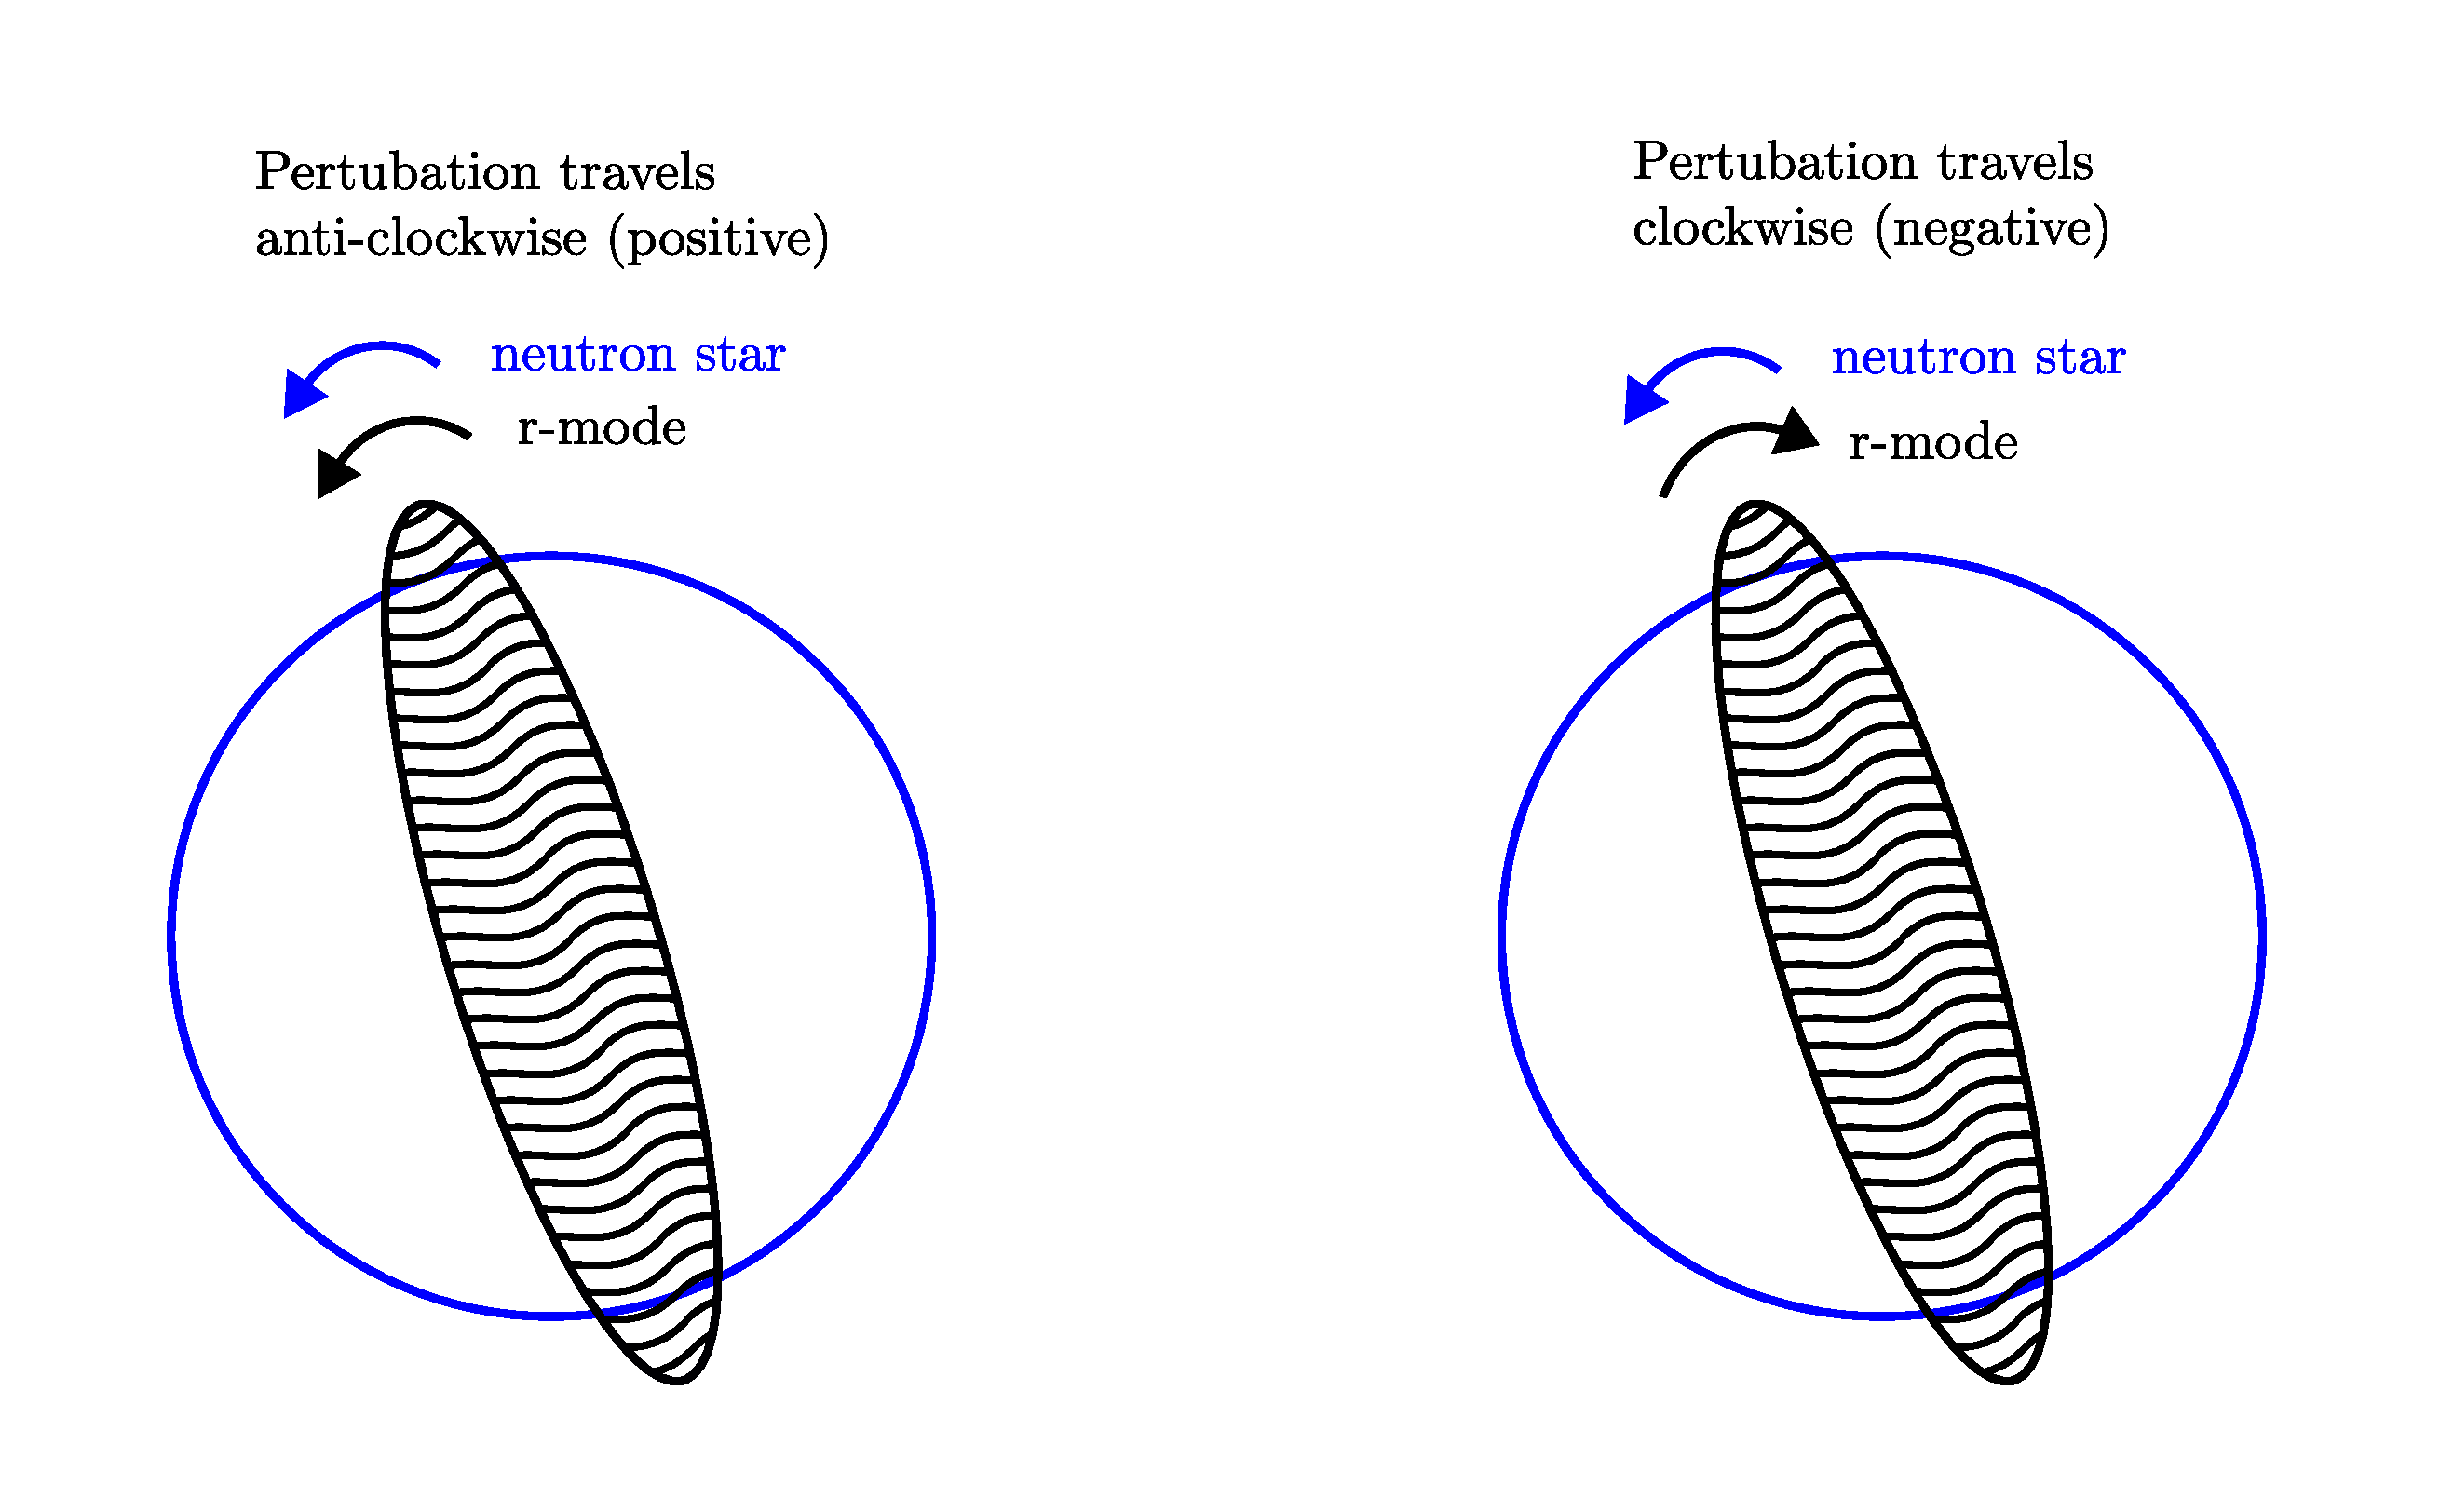
\includegraphics[width=\textwidth]{C1_intro/rmode.pdf}
	\caption[Generating \glspl{GW} from r-modes in neutron stars.]{The r-modes can travel in either direction in the star. in the case when the r-mode is moving clockwise and the neutron star is moving anti-clockwise, if the neutron star is rotating fast enough it can cause unstable emission of \gls{GW}. This image was reconstructed from \citep{jonesCFSInstability}.}
	\label{intro:source:cw:rmode}
\end{figure}
If these modes are excited in a non-rotating star, then they will emit \gls{GW} where the \gls{GW}  carries away angular momentum \citep{jonesCFSInstability}. 
For the mode travelling in a clockwise direction, this angular momentum is positive and the mode travelling anti-clockwise the angular momentum is negative. 
Therefore, the \gls{GW} is taking away either positive or negative angular momentum (adding angular momentum) depending on the direction of rotation.
The emission of \gls{GW} damps the modes and the magnitude of the perturbation decreases making them extremely difficult to detect.
Now if the neutron star is rotating, this can lead to an effect called the \gls{CFS} instability  \citep{chandrasekhar1970SolutionsTwo,friedman1978SecularInstability}. 
As the rotation speed of the neutron star increases, there are two different effects on the modes travelling in opposite directions. 
For the mode travelling anti-clockwise with the stars rotation, the mode will appear to be travelling faster, therefore, will emit more \gls{GW} taking away more angular momentum. This means that this mode will be damped more rapidly.
The interesting affect is for the mode travelling clockwise, opposite to the neutron stars rotation. 
At a certain rotation rate, the mode will be `frozen' from the observers perspective and no \gls{GW} will be emitted.
As the rotation rate increases further, the mode will appear to travel anti-clockwise to an observer, i.e. the mode is dragged in the opposite direction by the stars rotation. 
Here it is key to remember that this mode had negative angular momentum as in the neutron stars frame it is still travelling clockwise.
As the mode rotates its emits positive angular momentum, which is then subtracted from the modes negative angular momentum.
The magnitude of the angular momentum then increases such that more \glspl{GW} are released.
This effect causes the amplitude of the oscillation to grow and therefore become unstable.
Therefore, a neutron star is unstable to \gls{GW} emission if it is rotating sufficiently fast \citep{lasky2015GravitationalWaves}.
For a more detailed view on how r-modes generate \gls{GW} see \citep{owen1998GravitationalWaves,jonesCFSInstability}
\fi

%
% REMOVED LISA CW SOURCE FOR NOW
%
\if
To me \joe{either remove or rewrite the CBC LISA CWs}
Another potential source of \glspl{CW} is \gls{CBC} signals
early in the inspiral phase.  Before the final stages of the inspiral of a
\gls{CBC} signal, the objects orbiting at much slower non-relativistic
speeds.~\chris{these last 2 sentences need to be cleaned up/merged to make more
sense. The second sentence isn't really a sentence} They therefore emit a
\gls{GW} with a slowly varying frequency and can remain in this phase for
millions of years~\chris{too basic and vague. Are you sure it's not hundreds of
thousands? Do a calculation }.  This signal however, is at lower frequency than
ground based detectors can detect, therefore space based detectors such as
\gls{LISA} \citep{danzmann1996LISALaser} are expected to observe this type of
\gls{CW}.~\chris{OK, yes, but why start the sectiuon talking about a source
that isn't that important. Wouldn't it be better to discuss LISA CW sources at
the end. Plus the main LISA CW soiurce is white dwarf binaries.}
\fi

%%
%%  END OF REMOVED BIT
%%

%%%%%%%%%%%%%%%
%%%%%%%%%%%%%%
%%%%%%%%%%%%%%%
\section{\label{intro:detector}Detectors}
%%%%%%%%%%%%%%%%
%%%%%%%%%%%%%%
%%%%%%%%%%%%%%

The indirect detection of gravitational waves from the Hulse-Taylor binary
pulsar system \citep{weisberg1981GravitationalWaves} left little doubt that \gls{GW} existed.  The
real challenge was to design an instrument or develop a technique which could directly detect
gravitational waves, there were a number or proposed methods, notably: resonant bar detectors, both
ground based and space based interferometers, pulsar timing arrays and cosmic microwave background (CMB)
detectors. The first resonant bar detector was designed and built by Joseph
Weber \citep{weber1966ObservationThermal}, where they are large cylinders of metal
which resonate as a gravitational wave passes by.  There are a few different designs
of this type of detector, including an omni-directional design
\citep{dewaard2003MiniGRAILFirst}. 
Pulsar timing arrays aim to use the accurate arrival time of pulses
from millisecond pulsars to measure \gls{GW}
\citep{hobbs2017GravitationalWave}. As a \gls{GW} passes between the pulsar and
the observer, the arrival time of the pulses will change. The change in arrival time depends on the source and its parameters, however, for supermassive black hole binaries emitting at nanohertz frequencies at around 1 Gpc, the change in arrival time is by $\mathcal{O}(10)$ ns \citep{hobbs2017GravitationalWave}.  \gls{CMB} detectors can be used to find evidence of \gls{GW} by investigating the B-mode polarisations of the \gls{CMB}
\citep{ade2018ConstraintsPrimordial}. A number of
detectors are used to look at the \gls{CMB} however, are yet to
confirm a detection of a \gls{GW} signal.  
The current best known design of a \gls{GW} detector is the interferometer, the ground based detector \gls{LIGO}
made the first detection of \gls{GW} in 2015
\citep{abbott2016ObservationGravitational} and interferometers are being used for space based detectors.  These are the focus of this
section as the analysis that will follow uses data from the \gls{LIGO}
detectors in the USA \citep{abbott2009LIGOLaser,aasi2015AdvancedLIGO} and Virgo
detector in Italy
\citep{acernese2015AdvancedVirgo,acernese2008StatusVirgo}.~\chris{there are
potentially 3 or 4 paragraphs here if you were to expand on bar detectors, PTAs
and CMB measurements.} 

%%%%%%%%
%%%%%%%%%
\subsection{\label{intro:detector:ligo}Laser Interferometers}
%%%%%%%%%%
%%%%%%%%%

Laser interferometers use the interference of light to measure a
length change with high precision.  The majority of this
section will focus on ground based interferometers such as \gls{LIGO} and Virgo
\citep{aasi2015AdvancedLIGO,acernese2015AdvancedVirgo}.  A simple design of an
interferometer is shown in Fig.~\ref{detectors:interferometer:simple}, here a laser
beam is fired at a beam splitter which splits the light equally down two
perpendicular arms.  Each of these beams is reflected from a mirror at the end
of either arm, where the light then returns to the beam splitter where the two beams
are combined and sent to a photo-detector.  At the output, there is an
interference pattern between the two beams.  If the length of one of the arms
is changed then the interference pattern will change as the phase of one beam
changes with respect to the other.  The phase difference of the light can be
related to the wavelength of the light, $\lambda_l$ and the length of the
detectors arms $L$ by
%
\begin{equation}
\label{intro:detectors:phasechange}
\Delta \phi \sim 2 \pi \frac{\Delta L}{\lambda_l},
\end{equation}
%
where $\Delta
\phi$ is the phase change and $\Delta L$ is the difference in the arm lengths.
An interferometer can then measure small changes in the mirrors position.

\begin{figure}[hp]
    \centering
    \begin{subfigure}[h]{0.6\linewidth}
    	 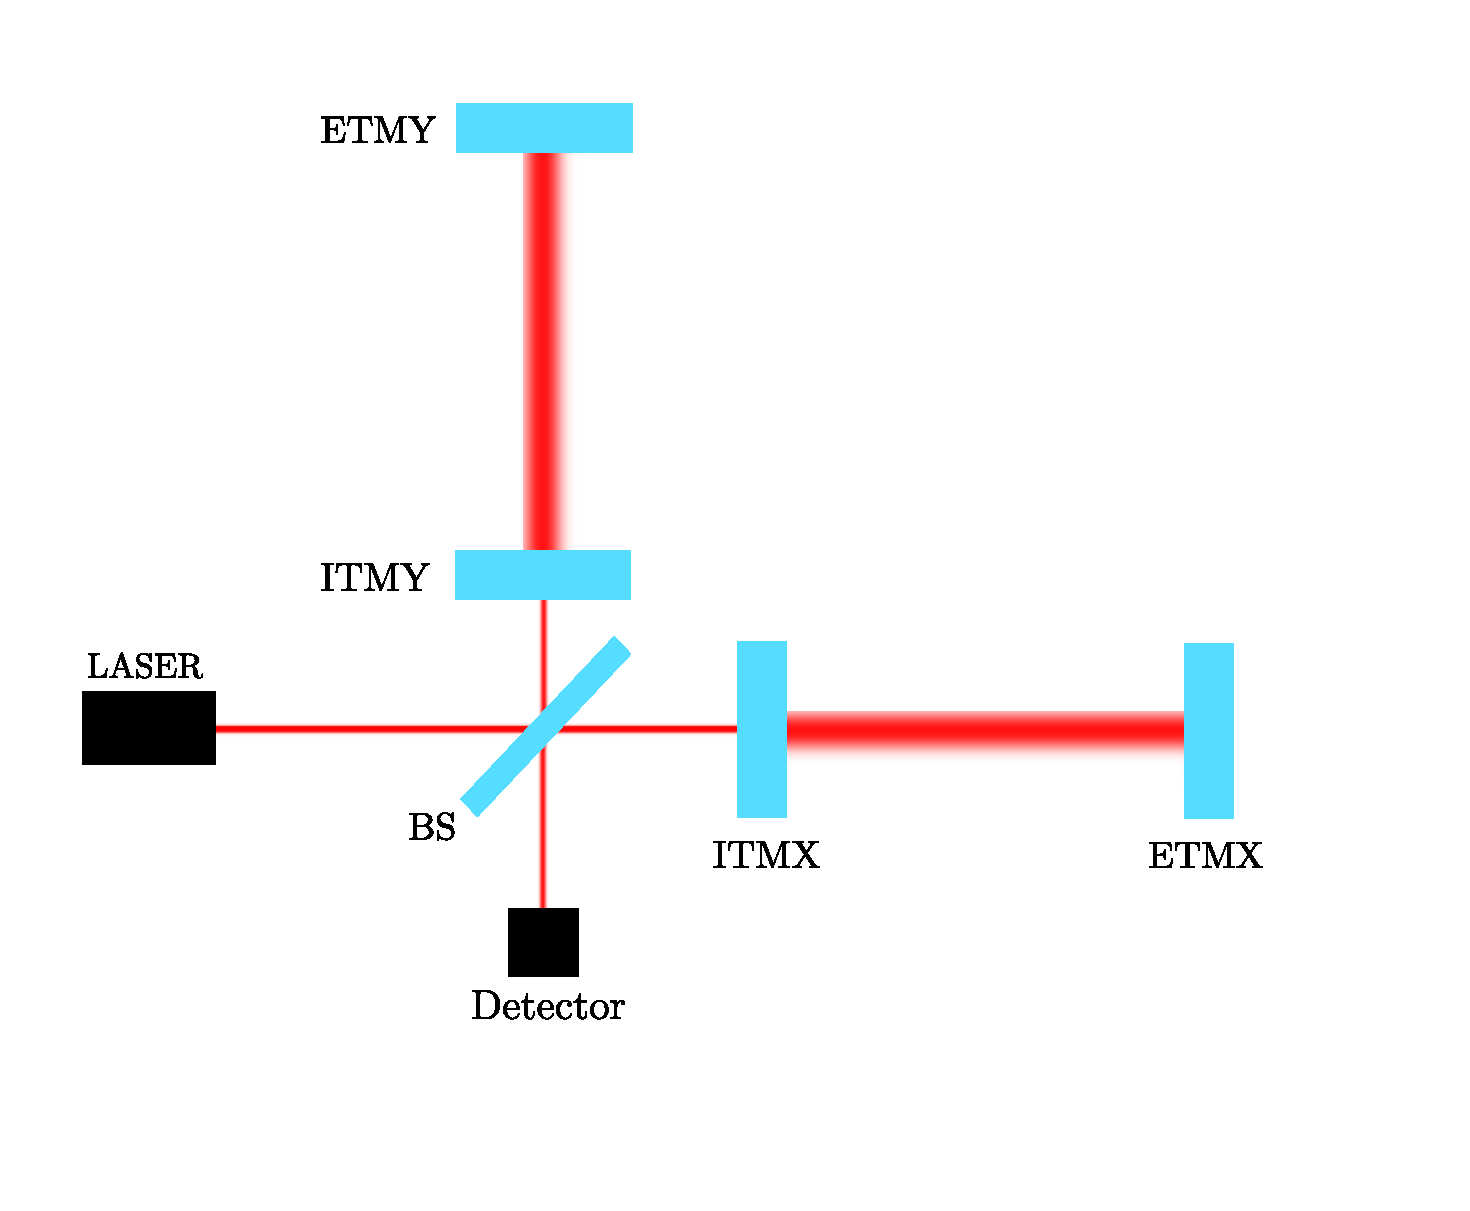
\includegraphics[width=\textwidth]{C1_intro/interferometer.pdf}
    	 \caption{Simple interferometer.}
    	 \label{detectors:interferometer:simple}
    \end{subfigure}
	\begin{subfigure}[h]{0.6\linewidth}
		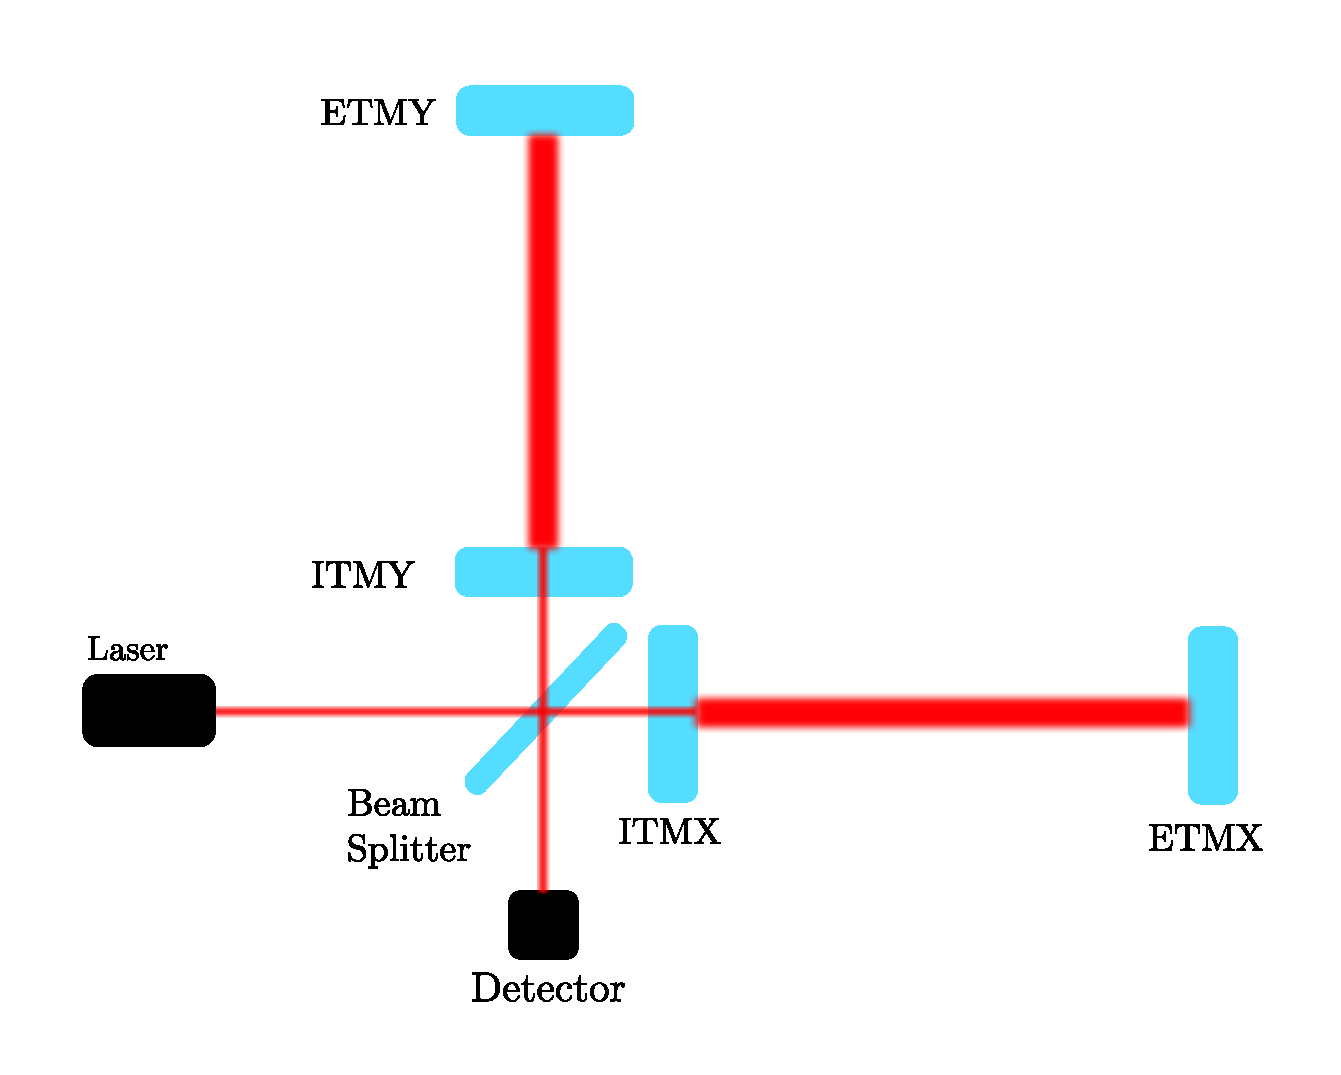
\includegraphics[width=\textwidth]{C1_intro/interferometer_fabry.pdf}
		\caption{Fabry-Perot interferometer.}
		\label{detectors:interferometer:fabry}
	\end{subfigure}
    \caption[Basic layout of the \gls{LIGO} detectors.]{Fig.~\ref{detectors:interferometer:simple} shows a basic interferometer. \gls{LIGO} includes many additions to this interferometer to increase its sensitivity to \gls{GW}, one addition known as a Fabry-Perot cavity is shown in Fig.~\ref{detectors:interferometer:fabry}.  \gls{ETMY} and \gls{ETMX} refer to the mirrors at the end of the interferometer arms.
\gls{ITMY} and \gls{ITMX} create a
Fabry-Perot cavity in the interferometers arms which can build up laser
power.}
\label{detectors:interferometer}
\end{figure}

This can be used in gravitational wave detection as the mirrors at the end of
each arm of the interferometer can be treated as `free' test masses.  Figure
\ref{gw:polarisations} shows the effect of a \gls{GW} on free test masses, where this can be seen by looking at the proper distance between two test masses.  If we
place two test masses along the $x$ axis ($\mu = 1$)with separation $L_0$ where a
gravitational wave is travelling along the $z$ axis ($\mu = 3$), the proper distance
between them is given by
%
\begin{equation}
    L = \int_{0}^{L_0} \sqrt{g_{\mu \nu} dx^{\mu} dx^{\nu}}= \int_{0}^{L_0} \sqrt{g_{11}} dx^1,
\end{equation}
%
where,
\begin{equation}
    \label{intro:detectors:metricpertubation}
     g_{11} = g_{xx} = 1 + h_{11} = 1 + h_{+}(t),
\end{equation}
which is the combination of Eq.~\ref{intro:gravwave:metric} and Eq.~\ref{intro:gw:gravwave}.  As $h_{+}(t) << 1$, is can be expanded to first order, i.e.  $\sqrt{g_{11}} = \sqrt{1 +
h_{+}(t)} \approx 1 + \frac{1}{2}h_{+}(t)$.  The proper distance is then
%
\begin{equation}
    \label{intro:detectors:properdist}
    \begin{split}
     L &\approx \int_{0}^{L_0} 1 + \frac{1}{2}h_{+}(t) dx \\
      &\approx L_0 + L_0 \frac{1}{2}h_{+}(t),
    \end{split}
\end{equation}
%
where here we use the long wavelength approximation, where we assume that the wave $h(t)$ does not change whilst the photon travels along the arm.
From Eq.~\ref{intro:detectors:properdist} on can see that in this configuration the
plus polarisation of the gravitational wave causes the separation between the
two test masses to oscillate \citep{flanagan2005BasicsGravitational}.  This
oscillation can then be expressed as a fractional length change
%
\begin{equation}
    \label{intro:detectors:fraclength}
    \frac{\delta L}{L_0} \approx \frac{1}{2} h_{+}.
\end{equation}
%
The fractional length change is then proportional to the \gls{GW}.

We can generalise Eq.~\ref{intro:detectors:properdist} slightly as in \citep{whelanGeometryGravitational} by defining the proper length measured along any axis defined by the vector $\bm{v} = v^i$, where in Eq.~\ref{intro:detectors:properdist} $v^i = (1,0,0)$, i.e. is along the $x$-axis.
Using $v^i = (1,0,0)$, the metric perturbation component $h_{11}$ in Eq.~\ref{intro:detectors:metricpertubation} can be generally in terms of the metric perturbation Eq.~\ref{intro:gw:gravwave} 
\begin{equation}
    h_{11} = v^i h_{ij} v^j,
\end{equation}
where, $i,j$ are the spatial indices of the metric.
From Eq.\ref{intro:detectors:properdist}, the length along some vector $\bm{v}$ can then be defined as 
\begin{equation}
    L_{\bm{v}} = L_0 + \frac{L_0}{2} h_{ij} v^i v^j.
\end{equation}
An interferometer measures the difference in length between two arms $\Delta L$, where we can define the arms along vector $\bm{v}$ and $\bm{u}$.
We can then write the difference in arm length along these vectors as
\begin{equation}
    \label{intro:detector:lengthdifference}
    \begin{split}
        \Delta L &= L_{\bm{v}} - L_{\bm{u}} = \frac{L_0}{2} \left( h_{ij} v^i v^j - h_{ij}u^i u^j \right) \\
                &= L_0\, h_{ij} \frac{ v^i v^j - u^i u^j }{2}\\
                &= L_0\, h_{ij} D^{ij},\\
    \end{split}
\end{equation}
where $D^{ij}$ is the detector tensor which depends on the detectors geometry \citep{whelanGeometryGravitational}.
The \gls{GW} strain is then the fractional difference in length of the arms
\begin{equation} 
    \label{intro:detectors:strain:detectortensor}
    h(t) = \frac{\Delta L(t)}{ L_0} = h_{ij}(t) D^{ij}.
\end{equation}

In practice, rather than measure the phase difference in Eq.~\ref{intro:detectors:phasechange} at the output of the detector, the position of the two mirrors are held in position such that the interference pattern is held on a dark fringe.
%
% The laser is on a dark fringe because whilst half way up a fringe would give the biggest change in power for a change in length, 
% the fluctuations in the power are much greater than the GW
% Instead, the laser phase is modulated such that the carrier is on a dark fringe and the sidebands are not.
% The GW is then encoded in the sidebands, therefore, the GW no longer competes with fluctuations at f_{GW} by at the frequency of modulation of the laser
% this is a much higher frequency (MHz) where the laser power fluctuations are lower as they follow 1/f 
%
The \gls{GW} strain is then proportional to the readout of the control systems $d(f)$ which hold the mirrors at this position \cite{ligoscientificcollaboration2017CalibrationAdvanced} 
\begin{equation}
    \tilde{h}(f) = T(f) \frac{d(f)}{L_0},
\end{equation}
where $T(f)$ is a transfer function which describes how the control systems affect the signal, for more details on this see \cite{ligoscientificcollaboration2017CalibrationAdvanced}.

If one looks at Eq.~\ref{intro:detectors:strain:detectortensor} then if the mirrors at the
end of the arms (\gls{ETMX} and \gls{ETMY}) are are placed
further from the beam splitter, i.e. $L_0$ is increased, then in the long wavelength approximation the length change
of the arms $\Delta L$ for the same \gls{GW} $h(t)$ will be greater.  Given that the interferometer measures $\Delta L$, this means that
increasing the length of the detectors arms increases the sensitivity of the
interferometer.  A method to achieve a similar affect without physically
increasing the arm length is to use a Fabry-Perot cavity
\citep{aasi2015AdvancedLIGO}, this is shown in
Fig.~\ref{detectors:interferometer:fabry}.  This is where a semi-transparent
mirror is placed between the beam splitter and end mirror in each arm (\gls{ITMX} and
\gls{ITMY}).  Light enters this cavity and reflects
back and forth between the two mirrors (\gls{ITMX} and \gls{ETMX}) a number of times before
returning to the beam splitter.  This increases the time the light spends in
one arm which is equivalent to increasing the arm length.  

As mentioned above, the interference pattern of is held on a dark fringe, this means that when a \gls{GW} is not present, the laser light will be reflected back to the input to the interferometer.
By placing a mirror between the beam splitter and the input laser, this light can be reflected back into the interferometer increasing the laser power in the arms \citep{pitkin2011GravitationalWave}, this is known as power recycling. The increase in power improves sensitivity of the detector by reducing the shot noise \citep{abbott2009LIGOLaser}, which is the statistical fluctuations associated with the discrete nature of photons. 
A technique which can be used to tune the detectors sensitivity to a smaller bandwidth is known as signal recycling. 
If a \gls{GW} is incident on the detector then it will cause sidebands in the laser light which will be visible at the output of the detector. By placing a mirror at this output, the sideband signal is`recycled' back into the arms increasing its \gls{SNR} \citep{pitkin2011GravitationalWave}. The bandwidth over which this signal can be recycled is governed by the reflectivity of the mirror, therefore, this can improve the sensitivity of the detector to specific bandwidths. 

Actual ground based \gls{GW} detectors such as \gls{LIGO} \citep{abbott2009LIGOLaser} and
Virgo \citep{acernese2015AdvancedVirgo} are much more complicated than
described above.  They use many techniques to increase the sensitivity some of
which are outlined in \citep{aasi2015AdvancedLIGO,abbott2009LIGOLaser}.  Many of these techniques are
designed to reduce non-astrophysical effects on the detector,
some of these effects and solutions are listed in
Sec.~\ref{intro:detector:noise}.

%%%%%%%%%%%
%%%%%%%%%%
\subsubsection{Detector response}
%%%%%%%%%%
%%%%%%%%%

The detectors are not equally sensitive to all polarisations to all locations on the sky, rather it has an antenna pattern which is dependent on the sky location and the polarisation of the \gls{GW}. 
We can find this antenna response of the detector as in \citep{maggioreGravitationalWaves}, by thinking about the \gls{GW} in the frame of the detector.
We can define the detector to be in the frame $(x,y,z)$ with the detector arms along the $x$ and $y$ axes, and the source to be in the frame $(x^{\prime},y^{\prime},z^{\prime})$, where the \gls{GW} is travelling along $z^{'}$ and is pointing towards the detector. 
The axes $z^{\prime}$ then has polar coordinates $\theta$ and $\phi$ in the detector frame.
We can determine the angular pattern functions by first looking at the spatial \gls{GW}, where the $h_{+}$ and $h_{\times}$ polarisations are defined with respect to the $(x^{\prime},y^{\prime},z^{\prime})$ frame
\begin{equation}
    \label{intro:detector:response:gwwave}
    h^{\prime}_{ij} = \left( 
    \begin{matrix} 
    h_{+} & h_{\times} & 0 \\
    h_{\times} & -h_{+} & 0 \\
    0 & 0 & 0  \\
    \end{matrix}
    \right).
\end{equation}
The frame of the source $(x^{\prime},y^{\prime},z^{\prime})$, can then be transformed into the detector frame using the rotation
\begin{equation}
    \label{intro:detector:response:rotation}
    \mathcal{R} = \left( 
    \begin{matrix} 
    \cos(\phi) & \sin(\phi) & 0 \\
    -\sin(\phi) & \cos(\phi) & 0 \\
    0 & 0 & 1  \\
    \end{matrix}
    \right)
    \left( 
    \begin{matrix} 
    \cos(\theta) & 0 & \sin(\theta) \\
    0 & 1 & 0 \\
    -\sin(\theta) & 0 & \cos(\theta)  \\
    \end{matrix}
    \right).
\end{equation}
This rotation matrix is then applied to the \gls{GW} twice as it is a tensor, i.e. $h_{ij} = \mathcal{R}_{il} \mathcal{R}_{jk} h^{\prime}_{lk} $ or in matrix notation $\bm{h} = \bm{\mathcal{R}} \bm{h}^{\prime} \bm{\mathcal{R}}^{T}$.

From Eq.\ref{intro:detector:lengthdifference}, we can see that the \gls{GW} strain measured by the detector $h(t)$ depends on the detector tensor, where if we take $v^i = (1,0,0)$ and $u^i = (0,1,0)$, i.e. the detectors arms are along the $x$ and $y$ axes the \gls{GW} strain becomes 
\begin{equation}
    \label{intro:detectors:strain:ligo}
    h(t) = \frac{1}{2} \left( h_{11} - h_{22} \right) = \frac{1}{2} \left( h_{xx} - h_{yy} \right),
\end{equation}
where we are then only interested in the $h_{xx}$ and $h_{yy}$ components of the \gls{GW} metric, \citep{maggioreGravitationalWaves}.
After applying the rotation tensor $\mathcal{R}$ in Eq.\ref{intro:detector:response:rotation} to the \gls{GW} metric in Eq.\ref{intro:gravwave:metric} this tensor, one can look at the $xx$ and $yy$ component of the signal
\begin{equation}
    \begin{split}
        h_{xx} &= \left[ \cos^2(\theta) \cos^2 (\phi) - \sin^2 (\phi)\right]h_{+} + 2\cos (\theta) \sin (\phi) \cos (\phi) h_{\times}\\
        h_{yy} &= \left[ \cos^2(\theta) \cos^2 (\phi) - \cos^2 (\phi)\right]h_{+} - 2\cos(\theta) \sin (\phi) \cos(\phi) h_{\times} . \\
    \end{split}
\end{equation}
From Eq.~\ref{intro:detectors:strain:ligo} we can write the \gls{GW} strain as
\begin{equation}
    \label{intro:detector:response:strain:polarisations}
    \begin{split}
        h(t) &= \frac{1}{2} \left[ 1 + \cos^2 \left(\theta\right) \right] \cos\left(2\phi\right) h_{+}(t) + \cos \left(\theta\right) \cos \left(2\phi \right)h_{\times}(t)\\
        &= F_{+}(\theta,\phi)h_{+}(t) + F_{\times}(\theta,\phi)h_{\times}(t),
    \end{split}
\end{equation}
where $F_{+}(\theta,\phi)$ and $F_{\times}(\theta,\phi)$ are the antenna pattern functions of the detector.
This is a a measure of how sensitive the detector is to different directions and polarisations. 

An example of the antenna response for a detector where the arms lie on the $x$ and $y$ axis is shown in Fig.~\ref{intro:detector:response:polarisations}.
%
\begin{figure}[h]
    \centering
    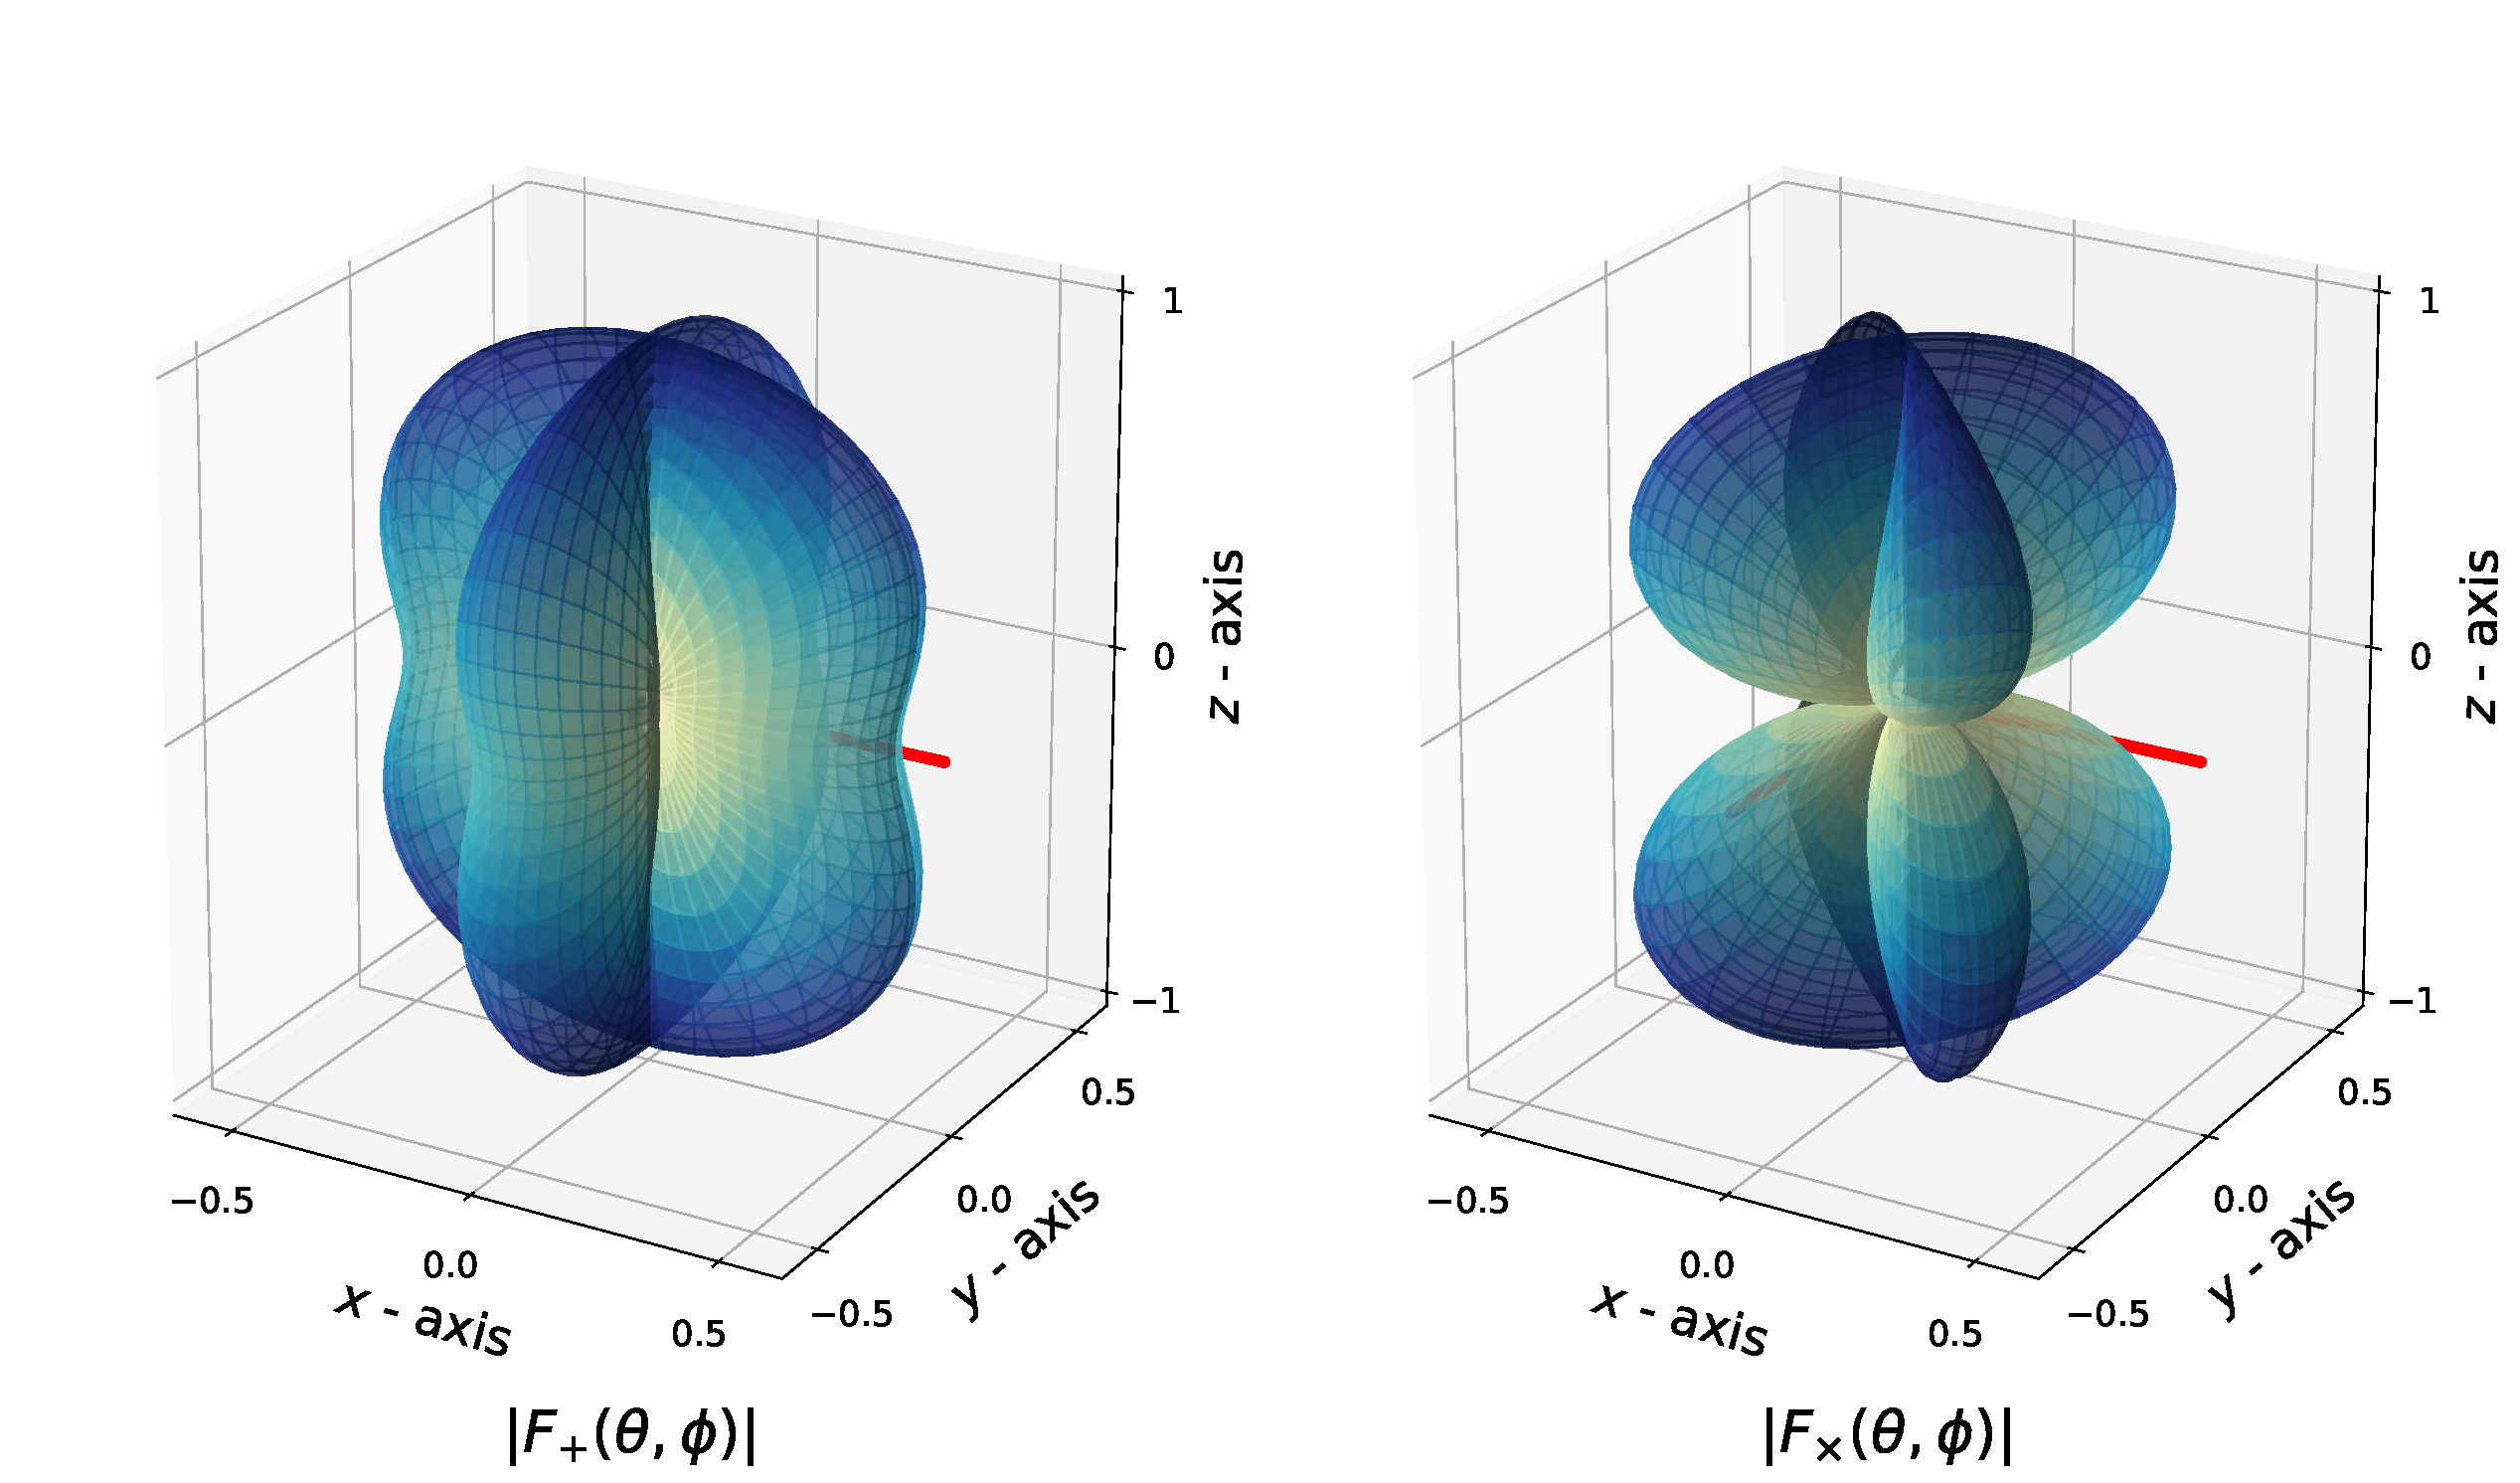
\includegraphics[width=\textwidth]{C1_intro/antenna_pattern.pdf}
    \caption[Antenna response of the \gls{LIGO} detectors.]{The antenna
response is shown for the plus and cross polarisations $F_{+}(\theta,\phi,\psi=0)$ and $F_{\times}(\theta,\phi,\psi=0)$ defined in Eq.~\ref{intro:detector:response:strain:polarisations} and Eq.~\ref{intro:detector:polarisationfuncs}. The detectors arms lie on the $x$ and
$y$ axis in the above plots. \joe{want to add a radial heatmap to make this clearerbut see if time}} \label{intro:detector:response:polarisations}
\end{figure}
%
The shape of the antenna pattern is clear when thinking about how a gravitational wave affects the test masses as in
Fig.~\ref{gw:polarisations}.
 As the \gls{GW} acts on test masses transverse to its propagation,
when the detector is face on to the source, there will be a maximum change in
the arm lengths and therefore a maximum sensitivity.  In the same way the
sensitivity will be at a minimum when edge to the source.
From some directions the \gls{GW} will change the length of the arms by the same amount, in these cases $\Delta L = 0$, therefore the detector is not sensitive to any \gls{GW} from that direction and this shows as the null areas in Fig.~\ref{intro:detector:response:polarisations} 

In the above example Eq.~\ref{intro:detector:response:strain:polarisations} we have defined the detectors frame (vectors $\bm{v}$ and $\bm{u}$) orthogonal to the propagation direction of the wave. 
We can however, define this more arbitrarily by performing a rotation $\psi$, known as the polarisation angle, in the plane transverse to the direction of propagation.
The \gls{GW} strain then becomes
\begin{equation}
	h(t) = F_{+}(\theta,\phi, \psi)h_{+}(t) + F_{\times}(\theta,\phi,\psi)h_{\times}(t),
\end{equation}
where the polarisation functions now depend on $\psi$ \citep{maggioreGravitationalWaves}
\begin{equation}
\label{intro:detector:polarisationfuncs}
	\begin{split}
	F_{+}(\theta,\phi,\psi) &= \frac{1}{2} \left[ 1 + \cos^2 \left(\theta\right) \right] \cos\left(2\phi\right) \cos{2\psi} + \cos \left(\theta\right) \cos \left(2\phi \right) \sin{2\psi} \\
	F_{\times}(\theta,\phi,\psi) &= \frac{1}{2} \left[ 1 + \cos^2 \left(\theta\right) \right] \cos\left(2\phi\right) \sin{2\psi} + \cos \left(\theta\right) \cos \left(2\phi \right) \sin{2\psi}
	\end{split}.
\end{equation}




%%%%%%%%%%%
%%%%%%%%%%
\subsubsection{\label{intro:detector:noise}Noise sources}
%%%%%%%%%%
%%%%%%%%%%

To sensitivity of the \gls{LIGO} detectors is limited by the combination of noise sources within the detector, where noise sources are any effect on the
output of the interferometer which is not from an astrophysical source.  
To increase the sensitivity of a detector, one needs to understand what causes certain noise features in the
detector, and how the effect of these can be limited.  
There are many sources of noise which can be broadly categorised into: fundamental noise, which is what ultimately limits the design sensitivity of the detector, technical noise which originates from sources such as electronics in the control systems and environmental noise which originates from the surrounding environments such as seismic motion \citep{martynov2016SensitivityAdvanced}.
Some of these noise sources and how they limit the detectors strain sensitivity
are all shown in Fig.~\ref{detectors:noisesensitivity} from
\citep{aasi2015AdvancedLIGO}, where in general different noise sources affect different areas of the frequency spectrum.

\begin{figure}[h]
    \centering
    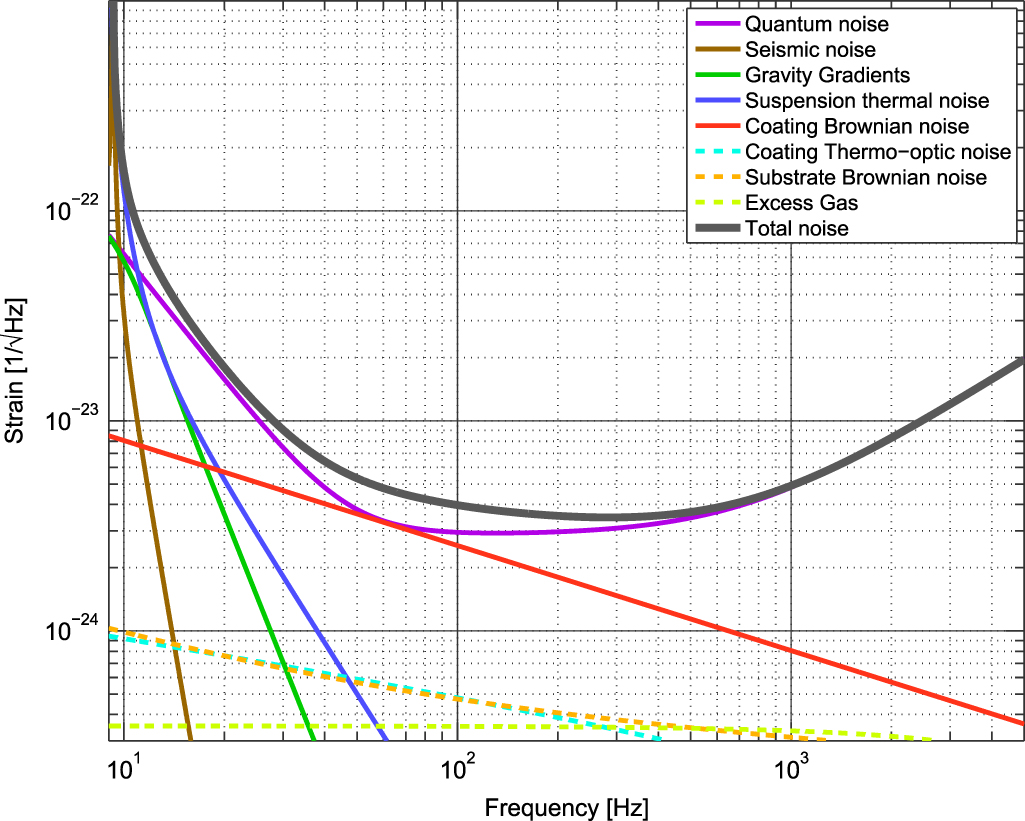
\includegraphics[width=0.9\textwidth]{C1_intro/noise_sensitivity.jpg}
    \caption[Example strain sensitivity curves for different noise sources in
\gls{LIGO}.]{The different noise sources affect the sensitivity of the
advanced \gls{LIGO} detectors at different frequencies, this figure shows a subset of the noise sources and how they limit the strain sensitivity of the detector \citep{aasi2015AdvancedLIGO}.}
\label{detectors:noisesensitivity} 
\end{figure}

Here I will summarise some of the limiting sources and also sources which
become useful for understanding later sections.

\begin{description}
\item[Seismic noise] This originates from vibrations in the Earth which can be from effects such as the Earths seismic
activity or anthropogenic sources, where this affects frequencies $\lesssim 20$ Hz in the \glspl{LIGO} spectrum. The oscillations originate
from a range of sources including earthquakes, ocean waves and traffic on nearby roads. They cause the mirrors to
oscillate and induce a change
in the length of the arm and therefore a change in the \gls{GW} readout channel. 
At the \gls{LIGO} sites, this causes the ground to move by about $10^{-9}\; \rm{m}/\sqrt{\rm{Hz}}$ at 10 Hz \citep{martynov2016SensitivityAdvanced}, which is orders of magnitude above the detectors design sensitivity. 
This is reduced by having multi-stage suspensions in the detectors which both actively and passively filter out the majority of seismic oscillations
\citep{matichard2015SeismicIsolation}.


\item[Thermal noise] This originates from mechanical systems where thermal motion can be transferred (coupled) into the measurement of the displacement of the test mass. There are a number of sources of this including the suspension thermal noise and the Brownian noise in the mirror coatings. 
The suspension thermal noise causes the test masses to move due to the thermal vibrations of the fibres suspending the test masses \citep{gonzalez2007HandbookApproximation}.
The coating Brownian noise is from thermal fluctuations in the layers of optical coating in the test masses \citep{martynov2016SensitivityAdvanced}. These effects are limited by using different coatings on the mirrors \citep{abernathy0OverviewResearch}.

\item[Quantum noise] Quantum noise originates from two main mechanisms: the shot noise associated with the
statistical uncertainty of the arrival time of photons at detector output, and the fluctuation in the radiation pressure noise associated with the momentum that photons transfer to the test masses \citep{aasi2013EnhancedSensitivity}.
The strain sensitivity limited by shot noise is defined in \citep{abbott2009LIGOLaser} as
\begin{equation}
	h(f) = \sqrt{\frac{\pi \hbar \lambda}{P c}} \frac{\sqrt{1 + (4 \pi f \tau_s)^2}}{4 \pi \tau_s},
\end{equation}
where $P$ is the power of the laser, $\lambda$ is the wavelength of the laser, $f$ is the \gls{GW} frequency, $\hbar$ is Planck's constant and $\tau_s$ is the arm cavity storage time. 
One can see from this that the shot noise decreases as the laser power increases, which is a reasons for the power recycling cavity described in Sec.~\ref{intro:detector:ligo}. 
This is a fundamental limit of the detectors sensitivity, however, there are methods which `cheat' this limit to reduce
the noise, for example using squeezed states of light \citep{aasi2013EnhancedSensitivity}. 

\item[Technical noise] Whilst this is not shown
in Fig.~\ref{detectors:noisesensitivity}, particular types of technical noise becomes important to searches
described later. An example of this is the noise generated by the digital and analogue electronics that are used to measure the signal and control the complex
detector system \citep{martynov2016SensitivityAdvanced}. Any fluctuations in the control system electronics can be transferred (coupled) into the measurement of the displacement of the test masses. 

\end{description}

There are also many other sources of noise including from fluctuations in the laser frequency and amplitude, jitter noise which is caused by motion of the mirrors that steer the laser, and Newtonian noise where variations in the density of matter surrounding the test mass changes the gravitational gradient \citep{martynov2016SensitivityAdvanced}.
For more discussion and detail of these noise sources and others see \citep{martynov2016SensitivityAdvanced,aasi2015AdvancedLIGO,aasi2015CharacterizationLIGO}. 
For the majority of this thesis there noise sources which cause narrowband spectral artefacts known as instrumental line provide the biggest challenge.  In Sec.~\ref{detchar} I will go into more detail
about these noise sources and
how they can be monitored and potentially removed.













